\documentclass[nobib,notoc,twoside,symmetric]{tufte-book}
\setcounter{tocdepth}{4}
\setcounter{secnumdepth}{4}

\usepackage{marginfix}
%to fix margins
\usepackage{multicol}
%for two-column.
\usepackage{CJKutf8}
%for mandarin

%\usepackage{scrextend} 
%\changefontsizes[11pt]{12pt}

\renewcommand{\footnotesize}{\small}

\geometry{a4paper,landscape,inner=30mm,top=15mm,bottom=10mm,headsep=\baselineskip,textwidth=170mm,marginparsep=8mm,marginparwidth=80mm,textheight=170mm,headheight=\baselineskip}

%\geometry{showframe}% for debugging purposes -- displays the margins

%\usepackage{stmaryrd}
%\usepackage{fontawesome}

\usepackage{amsmath,amsthm,amssymb,amsfonts}
\theoremstyle{definition}
\newtheorem{theorem}{Theorem}[section]
\newtheorem*{theorem*}{Theorem}
\newtheorem{corollary}[theorem]{Corollary}
\newtheorem{lemma}[theorem]{Lemma} 
\newtheorem{proposition}[theorem]{Proposition}
\newtheorem{conj}[theorem]{Conjecture}
\newtheorem{defn}[theorem]{Definition}
\newtheorem{fact}[theorem]{Fact} 
\newtheorem{example}[theorem]{Example} 
\newtheorem{examples}[theorem]{Examples}
\newtheorem{example*}[theorem]{Example*}
\newtheorem{examples*}[theorem]{Examples*}
\newtheorem{remark}[theorem]{Remark}
\newtheorem{remark*}[theorem]{Remark*}
\newtheorem{question}[theorem]{Question}
\newtheorem{assumption}[theorem]{Assumption}
\newtheorem{conjecture}[theorem]{Conjecture}
\newtheorem{convention}[theorem]{Convention}
\newtheorem{justification}[theorem]{Justification} 
\newtheorem{construction}[theorem]{Construction}
\newtheorem{rem}[theorem]{Reminder}
\newtheorem{intuition}[theorem]{Intuition}
\newtheorem{term}[theorem]{Terminology}
\newtheorem{scholium}[theorem]{Scholium}
\newtheorem{requirement}[theorem]{Requirement}
\newtheorem{notation}[theorem]{Notation}
\newtheorem{refinement}[theorem]{Refinement}
\newtheorem{thesis}[theorem]{Thesis}

%for fonts
\usepackage{newpxtext}
%\usepackage[fracspacing]{newpxmath}
\linespread{1.05}

\usepackage{tikz-cd}
\usepackage{macros/tikzfig}
\usepackage{macros/quiver}
\input{macros/thesis.tikzstyles}

% Set up the images/graphics package
\usepackage{graphicx}
\setkeys{Gin}{width=\linewidth,totalheight=\textheight,keepaspectratio}
\graphicspath{{graphics/}}

\title{String diagrams for text}
\author[V.W.]{Vincent Wang-Ma\'{s}cianica}
\date{\today}

% The following package makes prettier tables.  We're all about the bling!
\usepackage{booktabs}

% The units package provides nice, non-stacked fractions and better spacing
% for units.
\usepackage{units}

% The fancyvrb package lets us customize the formatting of verbatim
% environments.  We use a slightly smaller font.
\usepackage{fancyvrb}
\fvset{fontsize=\normalsize}

% Small sections of multiple columns
\usepackage{multicol}

% Squares
\usepackage{stix}

% Provides paragraphs of dummy text
\usepackage{lipsum}

% These commands are used to pretty-print LaTeX commands
\newcommand{\doccmd}[1]{\texttt{\textbackslash#1}}% command name -- adds backslash automatically
\newcommand{\docopt}[1]{\ensuremath{\langle}\textrm{\textit{#1}}\ensuremath{\rangle}}% optional command argument
\newcommand{\docarg}[1]{\textrm{\textit{#1}}}% (required) command argument
\newenvironment{docspec}{\begin{quote}\noindent}{\end{quote}}% command specification environment
\newcommand{\docenv}[1]{\textsf{#1}}% environment name
\newcommand{\docpkg}[1]{\texttt{#1}}% package name
\newcommand{\doccls}[1]{\texttt{#1}}% document class name
\newcommand{\docclsopt}[1]{\texttt{#1}}% document class option name

\usepackage{bussproofs}

\usepackage{xcolor}
\usepackage{xspace}
\def\bB{\begin{color}{blue}}
\def\bO{\begin{color}{orange}}
\def\bG{\begin{color}{green}}
\def\bM{\begin{color}{magenta}}
\def\e{\end{color}\xspace}

%For chesspieces
\usepackage{skak}

%For Brakets
\usepackage{physics}

\usepackage{xspace} 
%\usepackage{enumerate}
\usepackage{color} 
\def\bR{\begin{color}{red}}
\def\bB{\begin{color}{blue}}
\def\e{\end{color}\xspace}

%\usepackage{tocloft}
%\cftsetindents{section}{0em}{2em}
%\cftsetindents{subsection}{0em}{2em}
%\renewcommand\cfttoctitlefont{\hfill\Large\bfseries}
%\renewcommand\cftaftertoctitle{\hfill\mbox{}}

\begin{document}

\maketitle% this prints the handout title, author, and date

%\begin{fullwidth}
%\begin{multicols}{2}
\tableofcontents\marginnote{(Acknowledgements will go in a margin note here.)}
%\end{multicols}
%\end{fullwidth}


\chapter{Continuous relations for semantics}\label{chapter:contrel}
We want to reason formally with and about pictorial iconic representations, of the sort one might draw to solve a problem in elementary geometry stated in words, involving topological concepts such as \texttt{touching} and \texttt{inside}. To do this in string diagrams, I introduce and investigate the category of continuous relations, \textbf{ContRel}.
\section{Continuous Relations for iconic semantics}\label{sec:contrelintro}

\begin{figure}[h!]
\centering
\[\resizebox{\textwidth}{!}{\tikzfig{topology/conduitmetaphor}}\]
\caption{Sometimes it is very helpful to illustrate concepts using iconic representations in cartoons. For instance in the \emph{conduit metaphor} \citep{reddyConduitMetaphorCase}, \texttt{words} are considered \emph{containers} for \texttt{ideas}, and \texttt{communication} is considered a \emph{conduit} along which those containers are sent.}
\end{figure}

The aim of this chapter is to give us a formal setting in which we can paint pictures with words. More verbosely, to formalise cartoon doodles like the one above in a symmetric monoidal category so that we can give semantics to text circuits in terms of graphical, iconic representations -- cartoons, in short. To do so, we introduce the category \textbf{ContRel} of \emph{continuous relations}, which are a na\"{i}ve extension of the category \textbf{Top} of topological spaces and continuous functions towards continuous relations.\\

The main reason we prefer \textbf{ContRel} to either \textbf{Rel} or \textbf{Top} for our purposes is that we can diagrammatically characterise set-indexed collections of mutually disjoint open sets as \emph{sticky-spiders}: a generalisation of spiders that interact with idempotents. We can then treat the indexing set as a collection of labels, and an indexed open set as a doodle. Notably, spiders don't exist in cartesian \textbf{Top} except for the one-point space, and the spatial structure of open sets doesn't exist in \textbf{Rel}. But there are all kinds of poorly behaved open sets even on the plane, so enter the next benefit: In \textbf{ContRel}, we can diagrammatically characterise the reals as a topological space up to homeomorphism, which gives us a diagrammatic handle on paths and homotopies, mathematical concepts that enable us to diagrammatically characterise when open sets are connected, how they might move and transform continuously in space, and when open sets are contained inside others. And once we've formalised doodles we'll be able to treat ourselves to cartoons as formal semantics for language and nobody can stop us.

\newthought{Sidenote for category theorists}

The na\"{i}ve approach I take is to observe that the preimages of functions are precisely relational converses when functions are viewed as relations, so the preimage-preserves-opens condition that defines continuous functions directly translates to the relational case. To the best of my knowledge, the study of \textbf{ContRel} is a novel contribution. I venture two potential reasons.\\

First, it is because and not despite of the na\"{i}vity of the construction. Usually, the relationship between \textbf{Rel} and \textbf{Set} is often understood in sophisticated general methods which are inappropriate in different ways. I have tried applying Kliesli machinery which generalises to "relationification" of arbitrary categories via appropriate analogs of the powerset monad to relate \textbf{Top} and \textbf{ContRel}, but it is not evident to me whether there is such a monad. The view of relations as spans of maps in the base category should work, since \textbf{Top} has pullbacks, but this makes calculation difficult and especially cumbersome when monoidal structure is involved.\\

Second, the relational nature of \textbf{ContRel} means that the category has poor exactness properties. Even if the sophisticated machinery mentioned in the first reason manages to work, relational variants of \textbf{Top} are poor candidates for any kind of serious mathematics because they lack many limits and colimits. Since we take an entirely "monoidal" approach, we are able to find and make use of the rich structure of \textbf{ContRel} with a different toolkit.

\newpage
\clearpage
\clearmargin
\begin{fullwidth}

\section{Continuous Relations by examples}

Let's consider three topological spaces and examine the continuous relations between them. This way we can build up intuitions, and prove some tool results in the process.

The \textbf{singleton space} consists of a single point which is both open and closed. We denote this space $\bullet$. Concretely, the underlying set and topology is
\[(\{\star\} \ , \ \{\{\star\},\varnothing\})\] 
\ctikzfig{testspaces/singleton}

The \textbf{Sierpi\'{n}ski space} consists of two points, one of which (in yellow) is open, and the other (in cyan) is closed. We denote this space $\mathcal{S}$. Concretely, the underlying set and topology is:
\[\big( \{0,1\} \ , \ \{ \varnothing, \{ 1 \} , \{ 0,1\} \} \big)\]
\ctikzfig{testspaces/sierpinski}

The \textbf{unit square} has $[0,1] \times [0,1]$ as its underlying set.  Open sets are "blobs" painted with open balls. Points, lines, and bounded shapes are closed. We denote this space $\blacksquare$.
\ctikzfig{testspaces/unitsquare}
\end{fullwidth}

\newthought{$\bullet \rightarrow \bullet$:} There are two relations from the singleton to the singleton; the identity relation $\{ (\bullet,\bullet) \}$, and the empty relation $\varnothing$. Both are topological.

\newthought{$\bullet \rightarrow \mathcal{S}$:} There are four relations from the singleton to the Sierpi\'{n}ski space, corresponding to the subsets of $\mathcal{S}$. All of them are topological.


\newthought{$\mathcal{S} \rightarrow \bullet$:}
\marginnote{
\begin{example}[A noncontinuous relation]\label{ex:nontop}
The relation $\{(0,\bullet)\} \subset \mathcal{S} \times \bullet$ is not a continuous relation: the preimage of the open set $\{\bullet\}$ under this relation is the non-open set $\{0\}$.
\end{example}
}
There four candidate relations from the Sierpi\'{n}ski space to the singleton, but as we see in Example \ref{ex:nontop}, not all of them are topological.

\newthought{Now we need some abstraction.} We cannot study the continuous relations between the singleton and the unit square case by case. We discover that continuous relations out of the singleton indicate arbitrary subsets, and that continuous relations into the singleton indicate arbitrary opens.
\marginnote{
\begin{term}
Call a continuous relation $\bullet \rightarrow X^\tau$ a \textbf{state} of $X^\tau$, and a continuous relation $X^\tau \rightarrow \bullet$ a \textbf{test} of $X^\tau$.
\end{term}

\begin{proposition}\label{prop:states}
States $R: \bullet \rightarrow X^{\tau}$ correspond with subsets of $X$.
\begin{proof}
The preimage $R^\dag(U)$ of a (non-$\varnothing$) open $U \in \tau$ is $\star$ if $R(\star) \cap U$ is nonempty, and $\varnothing$ otherwise. Both $\star$ and $\varnothing$ are open in $\{\star\}^{\bullet}$. $R(\star)$ is free to specify any non-$\varnothing$ subset of $X$. The empty relation handles $\varnothing$ as an open of $X^{\tau}$.
\end{proof}
\end{proposition}

\begin{proposition}\label{prop:tests}
Tests $R: X^\tau \rightarrow \bullet$ correspond with open sets $U \in \tau$.
\begin{proof}
The preimage $R^\dag(\star)$ of $\star$ must be an open set of $X^\tau$ by definition \ref{defn:toprelation}. $R^\dag(\star)$ is free to specify any open set of $X^{\tau}$.
\end{proof}
\end{proposition}
}

\newthought{$\bullet \rightarrow \blacksquare$:} Proposition \ref{prop:states} tells us that there are as many continuous relations from the singleton to the unit square as there are subsets of the unit square.

\newthought{$\blacksquare \rightarrow \bullet$:} Proposition \ref{prop:tests} tells us that there are as many continuous relations from the unit square to the singleton as there are open sets of the unit square.

\newthought{There are 16 candidate relations $\mathcal{S} \rightarrow \mathcal{S}$ to check.} A case-by-case approach won't scale, so we could instead identify the building blocks of continuous relations with the same source and target space.

\newthought{Which relations $X^\tau \rightarrow Y^\sigma$ are always continuous?}

\newthought{The empty relation is always continuous.}
\marginnote{
    \begin{rem}[Empty relation]
    The \textbf{empty relation} $X \rightarrow Y$ relates nothing. It is defined:
    \[ \varnothing \subset X \times Y\]
    \end{rem}
}
\begin{proposition}
\label{prop:emptyrel}
\begin{proof}
The preimage of the empty relation is always $\varnothing$, which is open by definition.
\end{proof}
\end{proposition}

\newthought{Full relations are always continuous}
\marginnote{
    \begin{rem}[Full relation]
    The \textbf{full relation} $X \rightarrow Y$ relates everything to everything. It is all of $X \times Y$.
    \end{rem}
}
\begin{proposition}
\label{prop:fullrel}
\begin{proof}
The preimage of any subset of $Y$ -- open or not -- under the full relation is the whole of $X$, which is open by definition.
\end{proof}
\end{proposition}

\newthought{Full relations restricted to open sets in the domain are continuous.}
\begin{proposition}\label{prop:bowtie}
Given an open $U \subseteq X^\tau$, and an arbitrary subset $K \subset Y^\sigma$, the relation $U \times K \subseteq X \times Y$ is open.
\begin{proof}
Consider an arbitrary open set $V \in \sigma$. Either $V$ and $K$ are disjoint, or they overlap. If they are disjoint, the preimage of $V$ is $\varnothing$, which is open. If they overlap, the preimage of $V$ is $U$, which is open.
\end{proof}
\end{proposition}

\newthought{Continuous functions are always continuous.}
\begin{proposition}\label{prop:func}
If $f: X^\tau \rightarrow Y^\sigma$ is a continuous function, then it is also a continuous relation.
\begin{proof}
Functions are special cases of relations. The relational converse of a function viewed in this way is the same thing as the preimage.
\end{proof}
\end{proposition}

\newthought{The identity relation is always continuous.}
\marginnote{
    \begin{rem}[Identity relation]
    The \textbf{identity relation} $X \rightarrow X$ relates anything to itself. It is defined:
    \[ \{(x,x) : x \in X\} \subseteq X \times X\]
    \end{rem}
}
The identity relation is also the "trivial" continuous map from a space to itself, so this also follows from Proposition \ref{prop:func}.
\begin{proposition}\label{prop:idrel}
\begin{proof}
The preimage of any open set under the identity relation is itself, which is open by assumption.
\end{proof}
\end{proposition}

\newthought{Given two continuous relations $R,S : X^\tau \rightarrow Y^\sigma$, how can we combine them?}\marginnote{
\begin{rem}[Union, intersection, and ordering of relations]
Recall that relations $X \rightarrow Y$ can be viewed as subsets of $X \times Y$. So it makes sense to speak of the union and intersection of relations, and of partially ordering them by inclusion.
\end{rem}
}

\begin{proposition}\label{prop:framehom}
If $R,S: X^\tau \rightarrow Y^\sigma$ are continuous relations, so are $R \cap S$ and $R \cup S$.
\begin{proof}
Replace $\square$ with either $\cup$ or $\cap$. For any non-$\varnothing$ open $U \in \sigma$: \[(R \square S)^\dag (U) = R^\dag(U) \square S^\dag(U)\] As $R,S$ are continuous relations, $R^\dag(U),S^\dag(U) \in \tau$, so $R^\dag(U) \square S^\dag(U) = (R \square S)^\dag (U) \in \tau$. Thus $R\square S$ is also a continuous relation.
\end{proof}
\end{proposition}

\begin{corollary}\label{cor:homspace}
Continuous relations $X^\tau \rightarrow Y^\sigma$ are closed under arbitrary union and finite intersection. Hence, continuous relations $X^\tau \rightarrow Y^\sigma$ form a topological space where each continuous relation is an open set on the base space $X \times Y$, where the full relation $X \rightarrow Y$ is "everything", and the empty relation is "nothing".
\end{corollary}

\newthought{A topological basis for spaces of continuous relations}
\marginnote{
\begin{rem}[Topological Basis]
$\mathfrak{b} \subseteq \tau$ is a basis of the topology $\tau$ if every $U \in \tau$ is expressible as a union of elements of $\mathfrak{b}$. Every topology has a basis (itself). Minimal bases are not necessarily unique.
\end{rem}
}

\begin{defn}[Partial Functions]
A \textbf{partial function} $X \rightarrow Y$ is a relation for which each $x \in X$ has at most a single element in its image. In particular, all functions are special cases of partial functions, as is the empty relation.
\end{defn}

\begin{lemma}[Partial functions are a $\cap$-ideal]\label{lem:capideal}
The intersection $f \cap R$ of a partial function $f: X \rightarrow Y$ with any other relation $R: X \rightarrow Y$ is again a partial function.
\begin{proof}
Consider an arbitrary $x \in X$. $R(x) \cap f(x) \subseteq f(x)$, so the image of $x$ under $f \cap R$ contains at most one element, since $f(x)$ contains at most one element.
\end{proof}
\end{lemma}

\begin{marginfigure}
\centering
\scalebox{0.5}{\tikzfig{paintingexamples/sierandcanvas2_2}}
\caption{Regions of $\blacksquare$ in the image of the yellow point alone will be coloured yellow, and regions in the image of both yellow and cyan will be coloured green:}
\label{fig:yellowgreen}
\end{marginfigure}

\begin{lemma}[Any single edge can be extended to a continuous partial function]\label{lem:edgecomplete}
Given any $(x,y) \in X \times Y$, there exists a continuous partial function $X^\tau \rightarrow Y^\sigma$ that contains $(x,y)$.
\begin{proof}
Let $\mathcal{N}(x)$ denote some open neighbourhood of $x$ with respect to the topology $\tau$. Then $\{ (z,y) : z \in \mathcal{N}(x) \}$ is a continuous partial function that contains $(x,y)$.
\end{proof}
\end{lemma}

\begin{marginfigure}
\centering
\scalebox{0.5}{\tikzfig{paintingexamples/s2sqzoom}}
\caption{Regions in the image of the cyan point alone cannot be open sets by continuity, so they are either points or lines. Points and lines in cyan must be surrounded by an open region in either yellow or green, or else we violate continuity (open sets in red).}
\label{fig:cyan}
\end{marginfigure}

\begin{marginfigure}
\centering
\scalebox{0.75}{\tikzfig{paintingexamples/s2sqpainting}}
\caption{A continuous relation $\mathcal{S} \rightarrow \blacksquare$: "Flower and critter in a sunny field".}
\label{fig:flower}
\end{marginfigure}

\begin{marginfigure}
\centering
\scalebox{0.75}{\tikzfig{paintingexamples/sq2spainting}}
\caption{A continuous relation $\blacksquare \rightarrow \mathcal{S}$: "still math?". Black lines and dots indicate gaps.}
\label{fig:shitpost}
\end{marginfigure}

\begin{proposition}\label{prop:hombasis}
Continuous partial functions form a topological basis for the space $(X \times Y)^{(\tau \multimap \sigma)}$, where the opens are continuous relations $X^\tau \rightarrow Y^\sigma$.
\begin{proof}
We will show that every continuous relation $R: X^\tau \rightarrow Y^\sigma$ arises as a union of partial functions. Denote the set of continuous partial functions $\mathfrak{f}$. We claim that:
\[ R = \bigcup\limits_{F \in \mathfrak{f}} (R \cap F) \]
The $\supseteq$ direction is evident, while the $\subseteq$ direction follows from Lemma \ref{lem:edgecomplete}.
By Lemma \ref{lem:capideal}, every $R \cap F$ term is a partial function, and by Corollary \ref{cor:homspace}, continuous.
\end{proof}
\end{proposition}

\newthought{$\mathcal{S} \rightarrow \mathcal{S}$:} We can use Proposition \ref{prop:hombasis} to write out the topological basis of continuous partial functions, from which we can take unions to find all the continuous relations, which we depict in Figure \ref{fig:hassesierpinski}.

\newthought{$\mathcal{S} \rightarrow \blacksquare$:}
Now we use the colour convention of the points in $\mathcal{S}$ to "paint" continuous relations on the unit square "canvas", as in Figures \ref{fig:yellowgreen} and \ref{fig:cyan}. So each continuous relation is a painting, and we can characterise the paintings that correspond to continuous relations $\mathcal{S} \rightarrow \blacksquare$ in words as follows: Cyan only in points and lines, and either contained in or at the boundary of yellow or green. Have as much yellow and green as you like.

\newthought{$\blacksquare \rightarrow \mathcal{S}$:} The preimage of all of $\mathcal{S}$ must be an open set. So the painting cannot have stray lines or points outside of blobs. The preimage of yellow must be open, so the union of yellow and green in the painting cannot have stray lines or points outside of blobs. Point or line gaps within blobs are ok. Each connected blob can contain any colours in any shapes, subject to the constraint that if cyan appears anywhere, then either yellow or green must occur somewhere. Open blobs with no lines or points outside. Yellow and green considered alone is a painting made of blobs with no stray lines or points. If cyan appears anywhere, then either yellow or green have to appear somewhere.

\begin{figure}\label{fig:hassesierpinski}
\centering
\scalebox{0.5}{\tikzfig{testspaces/sierpinskienum}}
\caption{Hasse diagram of all continuous relations from the Sierpi\'{n}ski space to itself. Each relation is depicted left to right, and inclusion order is bottom-to-top. Relations that form the topological basis are boxed.}
\end{figure}

\clearpage

\newthought{One more example for fun: $[0,1] \rightarrow \blacksquare$:} We know how continuous functions from the unit line into the unit square look.
\begin{marginfigure}
\centering
\scalebox{0.5}{\tikzfig{paintingexamples/contline}}
\caption{
continuous functions $[0,1] \rightarrow \blacksquare$ follow the na\"{i}ve notion of continuity: a line one can draw on paper without lifting the pen off the page.
}
\label{fig:contline}
\end{marginfigure}
\newthought{Then what are the partial continuous functions?} If we understand these, we can obtain all continuous relations by arbitrary unions of the basis. Observe that the restriction of any continuous function to an open set in the source is a continuous partial function. The open sets of $[0,1]$ are collections of open intervals, each of which is homeomorphic to $(0,1)$, which is close enough to $[0,1]$.
%
\begin{marginfigure}
\centering
\scalebox{0.5}{\tikzfig{paintingexamples/contlines}}
\caption{
So a continuous partial function is \texttt{"(countably) many (open-ended) lines, each of which one can draw on paper without lifting the pen off the page."}
}
\label{fig:contline}
\end{marginfigure}
%
\begin{marginfigure}
\centering
\scalebox{0.5}{\tikzfig{paintingexamples/thickbrush}}
\caption{We can control the thickness of the brushstroke, by taking the union of (uncountably) many lines.}
\label{fig:thickbrush}
\end{marginfigure}

\newthought{Any painting is a continuous relation $[0,1] \rightarrow \blacksquare$.} By colour-coding $[0,1]$ and controlling brushstrokes, we can do quite a lot. Now we would like to develop the abstract machinery required to \emph{formally} paint pictures with words.

\begin{marginfigure}
\centering
\scalebox{0.8}{
\includegraphics{figures/paintingexamples/spectrum.png}}
\caption{Assign the visible spectrum of light to $[0,1]$. Colour open sets according to perceptual addition of light, computing brightness by normalising the measure of the open set.}
\end{marginfigure}

\begin{marginfigure}
\centering
\scalebox{0.8}{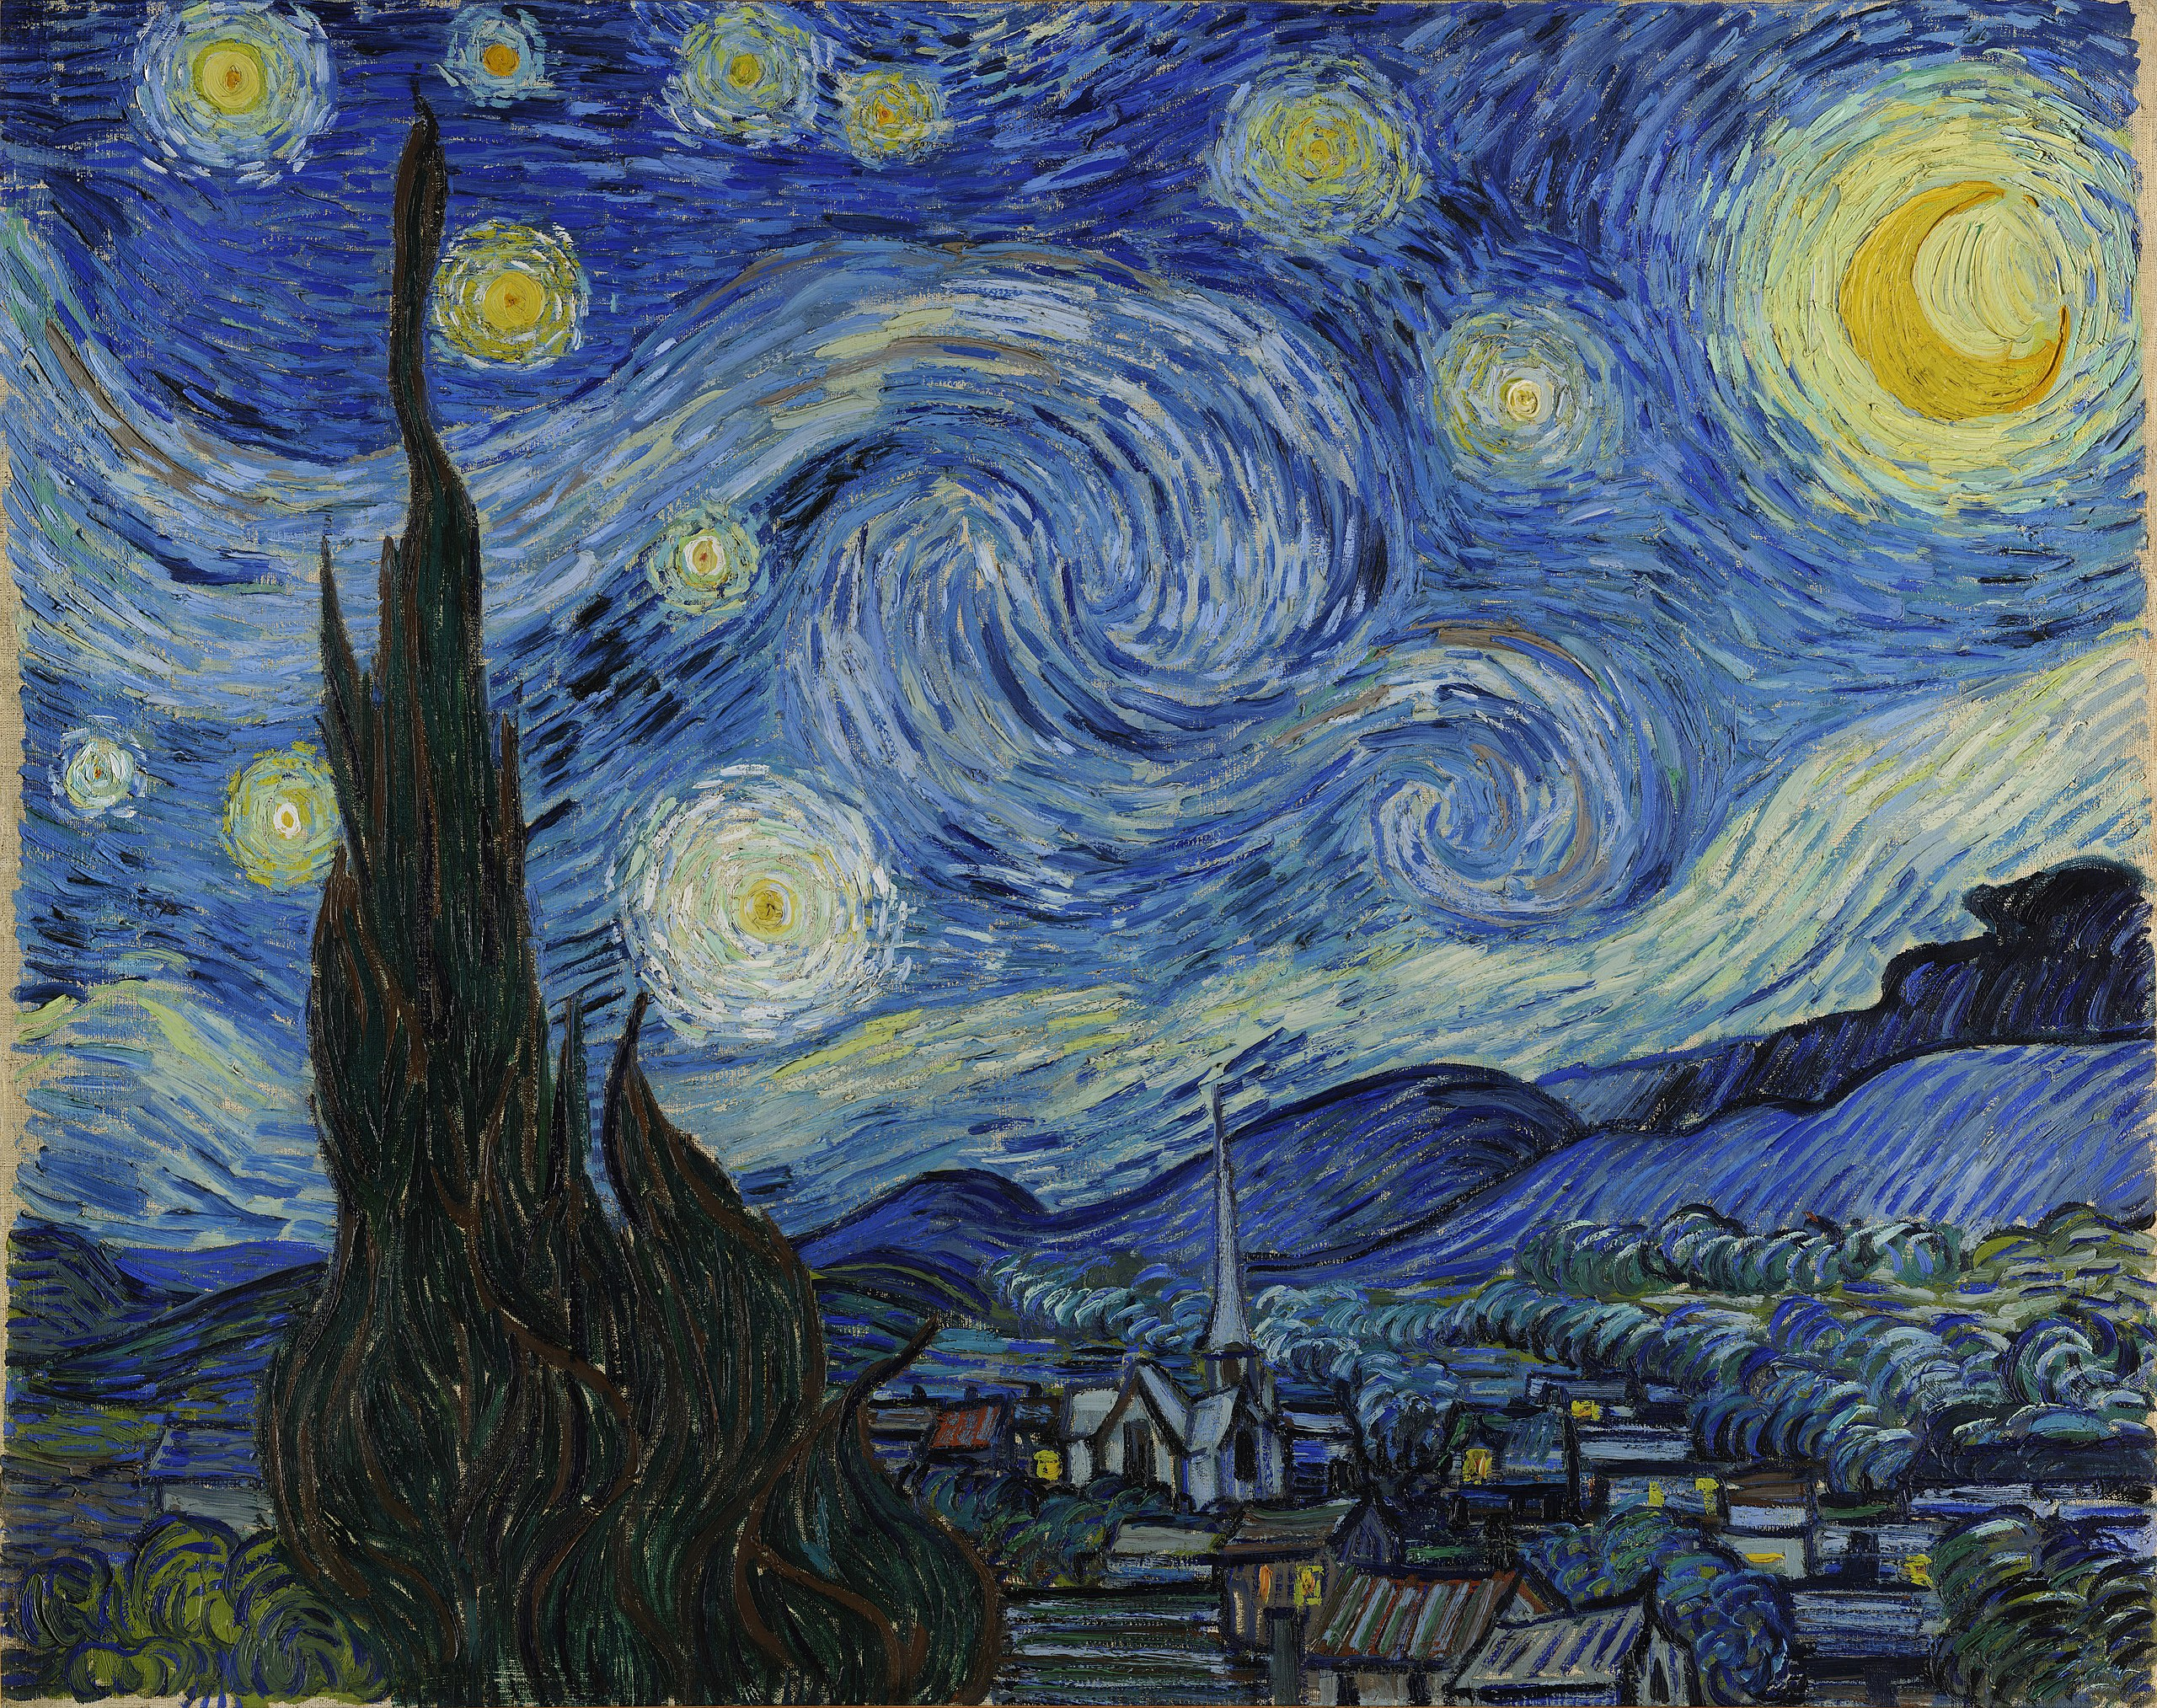
\includegraphics{figures/paintingexamples/starrynight}}
\caption{Like it or not, a continuous relation $[0,1] \rightarrow \blacksquare$: "The Starry Night", by Vincent van Gogh.}
\end{marginfigure}
\newpage
\clearpage
\clearmargin
\section{Continuous Relations}

\newthought{To the best of my knowledge, the study of \textbf{TopRel} is a novel contribution. I venture two potential reasons.}

\newthought{First, it is because and not despite of the na\"{i}vity of the construction.} Usually, the relationship between \textbf{Rel} and \textbf{Set} is often understood in sophisticated general methods which are inappropriate in different ways. I have tried applying Kliesli machinery which generalises to "relationification" of arbitrary categories via appropriate analogs of the powerset monad to relate \textbf{Top} and \textbf{TopRel}, but it is not evident to me whether there is such a monad. The view of relations as spans of maps in the base category should work, since \textbf{Top} has pullbacks, but this makes calculation difficult and especially cumbersome when monoidal structure is involved. The na\"{i}ve approach I take is to observe that the preimages of functions are precisely relational converses when functions are viewed as relations, so the preimage-preserves-opens condition that defines continuous functions directly translates to the relational case.

\newthought{Second, the relational nature of \textbf{TopRel} means that the category has poor exactness properties.} Even if the sophisticated machinery mentioned in the first reason do manage to work, relational variants of \textbf{Top} are poor candidates for any kind of serious mathematics because they lack many limits and colimits. Since we take an entirely "monoidal" approach -- a relative newcomer in terms of mathematical technique -- we are able to find and make use of the rich structure of \textbf{TopRel} with a different toolkit.\\

In the end, we want to formalise doodles, so perhaps there is some virtue in proceeding by elementary means.

\marginnote{
\begin{rem}[Topological Space]
A \emph{topological space} is a pair $(X,\tau)$, where $X$ is a set, and $\tau \subset \mathcal{P}(X)$ are the \emph{open sets} of $X$, such that:
\begin{description}
    \item["nothing" and "everything" are open]  \[\varnothing,X \in \tau\]
    \item[Arbitrary unions of opens are open] \[\{ U_i : i \in I \} \subseteq \tau \Rightarrow \bigcup\limits_{i \in I} U_i \in \tau \]
    \item[Finite intersections of opens are open] $n \in \mathbb{N}$: \[U_1,\cdots, U_n \in \tau \Rightarrow \bigcap\limits_{1\cdots, i , \cdots n} U_i \in \tau\]
\end{description}
\end{rem}
}

\marginnote{
\begin{rem}[Relational Converse]
Recall that a relation $R: S \rightarrow T$ is a subset $R \subseteq S \times T$. \[R^\dag : T \rightarrow S := \{ (t,s) : (s,t) \in R \}\]
\end{rem}
}

\marginnote{
\begin{rem}[Continuous function]
A function between sets $f: X \rightarrow Y$ is a continuous function between topologies $f: (X,\tau) \rightarrow (Y,\sigma)$ if \[U \in \sigma \Rightarrow f^{-1}(U) \in \tau\] where $f^{-1}$ denotes the inverse image.
\end{rem}
}

Recall that functions are relations, and the inverse image used in the definition of continuous maps is equivalent to the relational converse when functions are viewed as relations. So we can na\"{i}vely extend the notion of continuous maps to continuous relations between topological spaces.

\begin{defn}[Continuous Relation]\label{defn:toprelation}
A continuous relation $R: (X,\tau) \rightarrow (Y,\sigma)$ is a relation $R: X \rightarrow Y$ such that \[U \in \sigma \Rightarrow R^{\dag}(U) \in \tau\] where $\dag$ denotes the relational converse.
\end{defn}

\begin{notation}
For shorthand, we denote the topology $(X,\tau)$ as $X^{\tau}$. As special cases, we denote the discrete topology on $X$ as $X^{\star}$, and the indiscrete topology $X^{\circ}$.
\end{notation}

The symmetric monoidal structure is that of product topologies on objects, and products of relations on morphisms.

\marginnote{
\begin{rem}[Product Topology]
We denote the product topology of $X^\tau$ and $Y^\sigma$ as $(X \times Y)^{(\tau \times \sigma)}$. $\tau \times \sigma$ is the topology on $X \times Y$ generated by the basis $\{t \times s : t \in \mathfrak{b}_\tau, s \in \mathfrak{b}_\sigma\}$, where $\mathfrak{b}_\tau$ and $\mathfrak{b}_\sigma$ are bases for $\tau$ and $\sigma$ respectively.
\end{rem}
}

\marginnote{
    \begin{rem}[Product of relations]
    For relations between sets $R: X \rightarrow Y, S: A \rightarrow B$, the product relation $R \times S: X \times A \rightarrow Y \times B$ is defined to be \[ \{ ((x,a),(y,b)) : (x,y) \in R, (a,b) \in S \} \]
    \end{rem}
}

\begin{fullwidth}

\section{\textbf{TopRel} diagrammatically}

\subsection{Relations that are always continuous}

\newthought{Here are five continuous relations for any $X^\tau$:}

\[\scalebox{0.75}{\tikzfig{bestiary/generators}}\]

\newthought{Copy and delete obey the following equalities:}

\[\scalebox{0.75}{\tikzfig{bestiary/basicrelations}}\]

\newthought{The copy map can also be used to distinguish the deterministic maps -- points and functions -- which we notate with an extra dot.}

\[\scalebox{0.75}{\tikzfig{structure/determinism}}\]

\newthought{Everything, delete, nothing-states and nothing-tests combine to give two numbers, one and zero.} There are extra expressions in grey squares above: they anticipate the tape-diagrams we will later use to graphically express another monoidal product of \textbf{TopRel}, the direct sum $\oplus$.

\[\scalebox{0.75}{\tikzfig{bestiary/scalarrelations}}\]

\newthought{Zero scalars turn entire diagrams into zero morphisms.} There is a zero-morphism for every input-output pair of objects in \textbf{TopRel}. 

\[\scalebox{0.75}{\tikzfig{bestiary/zerorelations}}\]

\end{fullwidth}
\newpage
\clearpage
\clearmargin
\section{Populating space with shapes using sticky spiders}\label{sec:stickyspider}

%\begin{figure}\label{fig:spiderbicate}
%\scalebox{0.7}{\tikzfig{bestiary/spiderbicat}}
%\caption{The generators (in dashed boxes) and relations that make a spider. When the spider satisfies in addition the three inequalities b1-3, we call it a \textbf{relation-spider}.}
%\end{figure}

In this section, we seek to process-theoretically characterise disjoint collections of open sets of a space, so that we can play with doodles on the page as formal objects. It turns out that in \textbf{ContRel}, we can express them as idempotents that interact with spiders in a certain way.

\begin{example}[The copy-compare spiders of $\mathbf{Rel}$ are not always continuous]\label{ex:compnotspider}
The compare map for the Sierpi\'{n}ski space is not continuous, because the preimage of $\{0,1\}$ is $\{(0,0),(1,1)\}$, which is not open in the product space of $\mathcal{S}$ with itself.
\end{example}

\begin{rem}[copy-compare spiders of $\mathbf{Rel}$]
For a set $X$, the \emph{copy} map $X \rightarrow X \times X$ is defined:
\[\{(x,(x,x)) : x \in X \}\]
the \emph{compare} map $X \times X \rightarrow X$ is defined:
\[\{((x,x),x) : x \in X \}\]
These two maps are the (co)multiplications of special frobenius algebras. The (co)units are \emph{delete}:
\[\{(x,\star) : x \in X\}\]
and \emph{everything}:
\[\{(\star,x) : x \in X\}\]
\end{rem}

\newpage

\begin{myboxR}
\begin{proposition}\label{prop:copydiscrete}
The copy map is part of a special commutative frobenius algebra iff the topology is discrete.
\begin{proof}
Discrete topologies inherit the usual copy-compare spiders from \textbf{Rel}, so we have to show that when the copy map is part of a spider, the underlying wire must have a discrete topology. Suppose that some wire has a spider, and construct the following open set using an arbitrary point $p$:
\[\scalebox{0.5}{\tikzfig{structure/copyspiderproof/openpoint}}\]
It will suffice to show that this open set tests whether the input is the singleton $\{p\}$ -- when all singletons are open, the topology is discrete. As a lemma, we show that comparing distinct points $p \neq q$ yields the empty state.
\[\scalebox{0.5}{\tikzfig{structure/copyspiderproof/openpointproof}}\]
The (zero) implication follows since $p \neq q$ by assumption, so we know that deleting the comparison of $p$ and $q$ cannot be the unit scalar, and so must be the zero scalar, hence the comparison of $p$ and $q$ is the empty state. Now, the following case analysis shows that our open set only contains the point $p$.
\[\resizebox{0.75\textwidth}{!}{\tikzfig{structure/copyspiderproof/openpointcases}}\]
\end{proof}
\end{proposition}
\end{myboxR}

\begin{myboxB}
\begin{defn}[Sticky spiders]\label{defn:stickyspider}
A \textbf{sticky spider} (or just an $e$-spider, if we know that $e$ is a split idempotent), is a spider \emph{except} every identity wire on any side of an equation is replaced by the idempotent $e$.
\end{defn}

The desired graphical behaviour of a sticky spider is that one can still coalesce all connected spider-bodies together, but the 1-1 spider "sticks around" rather than disappearing as the identity. This is achieved by the following rules that cohere the idempotent $e$ with the (co)unit and (co)multiplications; they are the same as the usual rules for a special commutative frobenius algebra with two exceptions. First, where an identity wire appears in an equation, we replace it with an idempotent. Second, the monoid and comonoid components freely emit and absorb idempotents. By these rules, the usual proof [] for the normal form of spiders follows, except the idempotent becomes an explicit 1-1 spider, rather than the identity.
\[\resizebox{\textwidth}{!}{\tikzfig{structure/idemspider/stickyrelations}}\]
\end{myboxB}

\begin{myboxR}
\newthought{We can use split idempotents to transform copy-spiders from discrete topologies to sticky-spiders on other spaces.}
\begin{rem}[Split idempotents]
An \textbf{idempotent} in a category is a map $e: A \rightarrow A$ such that \[A \overset{e}{\rightarrow} A \overset{e}{\rightarrow} A = A \overset{e}{\rightarrow} A\]
A \textbf{split idempotent} is an idempotent $e: A \rightarrow A$ along with a \textbf{retract} $r: A \rightarrow B$ and a \textbf{section} $s: B \rightarrow A$ such that:
\[A \overset{e}{\rightarrow} A = A \overset{r}{\rightarrow} B \overset{s}{\rightarrow} A\]
\[B \overset{s}{\rightarrow} A \overset{r}{\rightarrow} B = B \overset{\mathop{id}}{\rightarrow} B\]
\end{rem}

We can graphically express the behaviour of a split idempotent $e$ as follows, where the semicircles for the section and retract $r,s$ form a visual pun. Recall that $X^\star$ denotes the discrete topology on the set $X$.

\[\scalebox{1}{\tikzfig{structure/idemspider/splitidem}}\]
\end{myboxR}

\begin{myboxB}
\begin{construction}[Sticky spiders from split idempotents]\label{cons:stickyfromsplit}
Given an idempotent $e: Y^\sigma \rightarrow Y^\sigma$ that splits through a discrete topology $X^\star$, we construct a new (co)multiplication as follows:
\[\scalebox{1}{\tikzfig{structure/idemspider/idemspiderv2}}\]
\end{construction}
\end{myboxB}

\begin{myboxR}
\begin{proposition}[Every idempotent that splits through a discrete topology gives a sticky spider]\label{prop:splitmeanssticky} The following is a sticky spider:
\[\scalebox{1}{\tikzfig{structure/idemspider/espiderstatement}}\]
\end{proposition}
We can check that Construction \ref{cons:stickyfromsplit} satisfies the frobenius rules as follows. We only present one equality; the rest follow the same idea.
\[\scalebox{1}{\tikzfig{structure/idemspider/espiderproofv2}}\]
\end{myboxR}
\begin{myboxR}
To verify the sticky spider rules, we first observe that since $X^\star \overset{s}{\rightarrow} Y^\sigma \overset{r}{\rightarrow} X^\star = X^\star \overset{\mathop{id}}{\rightarrow} X^\star$, $r$ must have all of $X^\star$ in its image, and $s$ must have all of $X^\star$ in its preimage, so we have the following:
\[\scalebox{1}{\tikzfig{structure/idemspider/splitonto}}\]
Now we show that e-unitality holds:
\[\scalebox{1}{\tikzfig{structure/idemspider/espiderproof2}}\]
The proofs of e-counitality, and e-speciality follow similarly.
\end{myboxR}

\begin{myboxB}
\newthought{We can prove a partial converse of Proposition \ref{prop:splitmeanssticky}:} we can identify two diagrammatic equations that tell us precisely when a sticky spider has an idempotent that splits though some discrete topology.
\begin{theorem}\label{thm:stickygraphical}
A sticky spider has an idempotent that splits through a discrete topology if and only if in addition to the sticky spider equalities, the following relations are also satisfied.
\[\scalebox{1}{\tikzfig{idemproof/unit-everything}} \quad\quad\quad\quad\quad\quad\quad\quad \scalebox{1}{\tikzfig{idemproof/comult-copy}}\]
\end{theorem}
The proof is involved, so here is a map of lemmas and propositions.
\[\resizebox{0.8\textwidth}{!}{\tikzfig{idemproof/claimmap2}}\]
\end{myboxB}

\begin{myboxR}
\begin{proposition}[comult/copy implies counit/delete]\label{prop:counitdelete}
\[\scalebox{1}{\tikzfig{idemproof/ecopy2delclaim}}\]
\begin{proof}
\[\scalebox{1}{\tikzfig{idemproof/ecopy2del}}\]
\end{proof}
\end{proposition}
\end{myboxR}

\begin{myboxB}
\begin{lemma}[All-or-Nothing]\label{lem:allornothing}
Consider the set $e(\{x\})$ obtained by applying the idempotent $e$ to a singleton $\{x\}$, and take an arbitrary element $y \in e(x)$ of this set. Then $e(\{y\}) = \varnothing$ or $e(\{x\}) = e(\{y\})$. Diagrammatically: \[\scalebox{0.75}{\tikzfig{idemproof/allornothingclaim}}\]
\end{lemma}
\[\scalebox{0.75}{\tikzfig{idemproof/allornothing2a}}\]
\end{myboxB}
\begin{myboxB}
\[\scalebox{0.75}{\tikzfig{idemproof/allornothing2b}}\]
\end{myboxB}

\begin{myboxR}
\begin{proposition}[$e$ of any point is $e$-copiable]\label{prop:epointcopy}
\[\scalebox{0.75}{\tikzfig{idemproof/pointidemcopiable}}\]
\begin{proof}
\[\scalebox{0.75}{\tikzfig{idemproof/pointidemcopiableproof}}\]
\end{proof}
\end{proposition}
\end{myboxR}

\begin{myboxB}
\begin{proposition}[The unit is the union of all $e$-copiables]\label{prop:copiablebasis}
\[\scalebox{0.8}{\tikzfig{idemproof/copiablebasisclaim}}\]
\begin{proof}
\[\scalebox{0.8}{\tikzfig{idemproof/copiablebasis}}\]
\end{proof}
\end{proposition}
\end{myboxB}

\begin{myboxR}
\begin{proposition}[$e$-copiable decomposition of $e$]\label{prop:decompidem}
\[\scalebox{1}{\tikzfig{idemproof/decompidemclaim}}\]
\begin{proof}
\[\scalebox{1}{\tikzfig{idemproof/decompidem}}\]
\end{proof}
\end{proposition}
\end{myboxR}

\begin{myboxB}
\begin{proposition}[$e$-copiable decomposition of counit]\label{prop:decompcounit}
\[\scalebox{1}{\tikzfig{idemproof/decompcounitclaim}}\]
\begin{proof}
\[\scalebox{1}{\tikzfig{idemproof/decompcounit}}\]
\end{proof}
\end{proposition}
\end{myboxB}

\begin{myboxR}
\newthought{The $e$-copiable states really do behave like an orthonormal basis, as the following Lemmas show.}
\begin{lemma}[$e$-copiables are orthogonal under multiplication]\label{lem:match}
\[\scalebox{0.75}{\tikzfig{idemproof/matchclaim}}\]
\begin{proof}
\[\scalebox{0.75}{\tikzfig{idemproof/match}}\]
\end{proof}
\end{lemma}
\end{myboxR}

\begin{myboxB}
\begin{convention}[Shorthand for the open set associated with an $e$-copiable]
We introduce the following diagrammatic shorthand.
\[\scalebox{1}{\tikzfig{idemproof/openshorthand}}\]
Including the coloured dot is justified, because these open sets are co-copiable with respect to the multiplication of the sticky spider.
\[\scalebox{1}{\tikzfig{idemproof/shorthandjustification}}\]
\end{convention}
\end{myboxB}

\begin{myboxR}
\begin{lemma}[Co-match]\label{lem:comatch}
\[\scalebox{1}{\tikzfig{idemproof/comatchclaim}}\]
\begin{proof}
\[\scalebox{0.9}{\tikzfig{idemproof/comatch}}\]
The claim then follows by applying Lemma \ref{lem:match} to the final diagram.
\end{proof}
\end{lemma}
\end{myboxR}

\begin{myboxB}
\begin{lemma}[e-copiables are e-fixpoints]\label{lem:ecopyfixpoint}
\[\scalebox{1}{\tikzfig{idemproof/dotcopyableclaim}}\]
\begin{proof}
\[\scalebox{1}{\tikzfig{idemproof/dotcopyable}}\]
Observe that the final equation of the proof also holds when the initial e-copiable is the empty set.
\end{proof}
\end{lemma}
\end{myboxB}

\begin{myboxR}
\begin{lemma}[$e$-copiables are normal]\label{lem:ecopynormal}
\[\scalebox{1}{\tikzfig{idemproof/copynormalclaim}}\]
\begin{proof}
\[\scalebox{1}{\tikzfig{idemproof/copynormal}}\]
\end{proof}
\end{lemma}
\end{myboxR}

\begin{myboxB}
\begin{proposition}[$e$-copiable decomposition of multiplication]\label{prop:decompmult}
\[\scalebox{1}{\tikzfig{idemproof/decompmultclaim}}\]
\begin{proof}
\[\scalebox{1}{\tikzfig{idemproof/decompmult}}\]
\end{proof}
\end{proposition}
\end{myboxB}

\begin{myboxR}
\begin{proposition}[$e$-copiable decomposition of comultiplication]\label{prop:decompcomult}
\[\scalebox{1}{\tikzfig{idemproof/decompcomultclaim}}\]
\begin{proof}
\[\scalebox{1}{\tikzfig{idemproof/decompcomult}}\]
\end{proof}
\end{proposition}
\end{myboxR}

\begin{myboxB}
\newthought{Now we can prove Theorem \ref{thm:stickygraphical}.}
First a reminder of the claim; we want to show that when given a sticky spider, the following relations hold if and only if the idempotent splits through a discrete topology.
\[\scalebox{0.8}{\tikzfig{idemproof/unit-everything}} \quad\quad\quad\quad\quad\quad\quad\quad \scalebox{0.8}{\tikzfig{idemproof/comult-copy}}\]
The crucial observation is that the $e$-copiable decomposition of the idempotent given by Proposition \ref{prop:decompidem} is equivalent to a split idempotent though the set of $e$-copiables equipped with discrete topology.
\[\scalebox{0.8}{\tikzfig{idemproof/finalproof}}\]
By copiable basis Proposition \ref{prop:copiablebasis} and the decompositions Propositions \ref{prop:decompcounit}, \ref{prop:decompmult}, \ref{prop:decompcomult}, we obtain the only-if direction.
\[\scalebox{0.8}{\tikzfig{idemproof/finalproof2}}\]
\end{myboxB}
\begin{myboxB}
The if direction is an easy check. For the unit/everything relation, we have:
\[\scalebox{0.8}{\tikzfig{idemproof/finalproof3}}\]
For the counit/delete relation, we observe that for any split idempotent, the retract must be a partial function. To see this, suppose the split idempotent $e = r;s$ is on $(X,\tau)$ and the discrete topology is $Y^\star$. Seeking contradiction, if the retract is not a partial function, then there is some point $x \in X$ such that $x \in e(x)$, and the image $I := r(x) \subseteq Y$ contains more than one point, which we denote and discriminate $a,b \in r(x) \subseteq Y$ and $a \neq b$. Because the composite $s;r = 1_Y$ of the section and retract must recover the identity on $Y^\star$, the section $s$ must be total -- i.e. the image $s(X) = Y$. So $x \in s(a) \cap s(b)$. Now we have that $(a,x),(b,x) \in s$, and $(x,a),(x,b) \in r$, therefore $(a,b),(b,a) \in s;r$, which by $a \neq b$ contradicts that $s;r$ is the identity relation $1_Y$.
\[\scalebox{0.8}{\tikzfig{idemproof/finalproof4}}\]
\end{myboxB}

\begin{myboxR}
\begin{defn}[Labels, shapes, cores, halos]
Recall by Proposition \ref{prop:decompidem} that we can express the idempotent as a union of continuous relations formed of a state and test, for some indexing set of \emph{labels} $\mathcal{L}$.
\[\tikzfig{topology/shape1}\]
A \emph{shape} is a component of this union corresponding to some arbitary $l \in L$. So we refer to a sticky spider as a labelled collection of shapes. The state of a shape is the \emph{halo} of the shape. The halos are precisely the copiables of the sticky spider. The test of a shape is the \emph{core}. The cores are precisely the cocopiables of the sticky spider.
\[\tikzfig{topology/shape2}\]
\end{defn}
\end{myboxR}

\begin{myboxB}
\begin{proposition}[Core exclusion: Distinct cores cannot overlap]\label{prop:core-core-exclusion}
\begin{proof}
A direct consequence of Lemma \ref{lem:comatch}.
\end{proof}
\end{proposition}
\end{myboxB}

\begin{myboxR}
\begin{proposition}[Core-halo exclusion: Each core only overlaps with its corresponding halo]\label{prop:core-halo-exclusion}
\begin{proof}
Seeking contradiction, if a core overlapped with multiple halos, Lemma \ref{lem:ecopyfixpoint} would be violated.
\end{proof}
\end{proposition}
\end{myboxR}

\begin{myboxB}
\begin{proposition}[Halo non-exclusion: halos may overlap]
\begin{proof}
By example:
\[\tikzfig{topology/halooverlap}\]
The two shapes are colour coded cyan and magenta. The halos are two triangles which overlap at a yellow region, and partially overlap with their blobby cores. The cores are outlined in dotted blue and orange respectively. Observe that cores and halos do not have to be simply connected; in this example the core of the magenta shape has two connected components. Viewing these sticky spiders as a process, any shape that overlaps with the magenta core will be deleted and replaced by the magenta triangle, and similarly with the cyan cores and triangle. Any shape that overlaps with both the magenta and cyan cores will be deleted and replaced by the union of the triangles. Any shape that overlaps with neither core will be deleted and not replaced.
\end{proof}
\end{proposition}
\end{myboxB}

\begin{myboxR}
\begin{corollary}[Only opens please]
A sticky spider corresponds to a set-indexed disjoint collection of open sets when, in addition to the equations of Theorem \ref{thm:stickygraphical}, it satisfies one more, depicted below on the left.
\[\scalebox{1}{\tikzfig{idemproof/opensonly}}\]
Observe that the right hand equation above is precisely what we want expressed in diagrams: that every halo matches its core. For the forward direction, we have:
\[\scalebox{1}{\tikzfig{idemproof/opensonly3}}\]
\end{corollary}
\end{myboxR}

\begin{myboxR}
For the backward direction, we rely on the fact that cores are non-empty (or else we would fail to satisfy the identity equation of the split idempotent) to eliminate the floating scalars.
\[\scalebox{1}{\tikzfig{idemproof/opensonly2}}\]
By Proposition \ref{prop:core-core-exclusion}, we have disjointness.\\

So, without loss of generality, we may treat any collection of disjoint open shapes on a page as a sticky spider.
\end{myboxR}

\clearpage
\newpage
\clearpage
\clearmargin
\section{Basic topological concepts in flatland via \textbf{ContRel}}\label{sec:concepts}

The goal now is to demonstrate the use of the sticky spiders we have obtained in the previous section as formal semantics for the kinds of schematic doodles or cartoons we would like to draw. Throughout we consider sticky spiders on $\mathbb{R}^2$. In service of defining \emph{configuration spaces} of shapes up to rigid displacement, we diagrammatically characterise the topological subgroup of isometries of $\mathbb{R}^2$ by building up in the diagrammatic presentations of the unit interval, metrics, and topological groups. To further isolate rigid displacements that arise from continuous sliding motion of shapes in the plane (thus excluding displacements that result in mirror-images), we diagrammatically characterise an analogue of homotopy in the relational setting. Finally, in we build up a stock of topological concepts and study by examples how implementing these concepts within text circuits explains some idiosyncrasies of the theory: namely why noun wires are labelled by their noun, why adjective gates ought to commute, and why verb gates do not.

\newthought{Itinerary of upcoming examples and definitions:} I would like to say it's obvious how to make shapes move and tell when they are touching and so on, but you may not believe me. So, I am going to recover a fair chunk of elementary topology diagrammatically in \textbf{ContRel}.

\newthought{Shapes and places} We can already do interesting things with just sticky spiders. In Example \ref{ex:chessboard}, we show how we can use sticky spiders to tell how pieces are on a chessboard. How is it that pieces on a chessboard in \emph{continuous} space are translated into \emph{discrete} data, such as \texttt{pawn on e4}?

\newthought{The reals}
To begin modelling more complex concepts, we first need to extend our topological tools. The first stop is the reals. There are many spaces homeomorphic to the real line. How do we know when we have one of them? The following theorem provides an answer:
\begin{theorem}[Friedman]\label{thm:Friedman}
Let $\big((X,\tau), < \big)$ be a topological space with a total order. If there exists a continuous map $f: X \times X \rightarrow X$ such that $\forall a,b_{\in X} : a < f(a,b) < b$, then $X$ is homeomorphic to $\mathbb{R}$. \citep{friedman_fom_2005}
\end{theorem}
We diagrammatically characterise total orders in Definition \ref{defn:lessthan}. Here Trichotomy requires us to appeal to the rig structure so that we can access unions of processes explicitly. Going forward we will also introduce quantifiers into process-theoretic equations, essentially treating process-equations as we would any other symbolic algebraic specification. Then we express Friedman's theorem using diagrammatic equations in Definition \ref{defn:friedfunct}.

\newthought{The unit interval}
If we have the unit interval, we can begin to define what it would mean for spaces to be connected (by drawing lines between points in those spaces), and we can also move towards defining motion as movement along a line. To obtain the unit interval (up to homeomorphism) we need to add endpoints to $\mathbb{R}$. We can introduce endpoints for open intervals directly by asking for the space $X$ to have points that are less than or greater than all other points. Another method, which we will use here for primarily aesthetic reasons, is to use endocombinators to define suprema. For a motivating example of the ubiquity of endocombinators, consider the case when we have a locally indiscrete topology:
\begin{defn}[Locally indiscrete topology]
$(X,\tau)$ is \emph{locally indiscrete} when every open set is also closed.
\end{defn}
If we know that a topology is locally indiscrete and we are given an open $U$, we would like to notate the complement $X/U$ -- which we know to be open -- as any of the following, which only differ up to notation.
\[\resizebox{0.5\textwidth}{!}{\tikzfig{topology/negbubble}}\]
Unfortunately, the complementation operation $X/-$ is not in general a continuous relation, hence in the lattermost expression above we resort to using bubbles -- endocombinators -- as syntactic sugar. Endocombinators are like functional expressions applied to diagrams: the semantics and notation for which we borrow and modify from \citep{haydon_compositional_2020}.
\begin{defn}[Partial endocombinator]
In a category $\mathcal{C}$, a \emph{partial endocombinator} on a homset $\mathcal(C)(A,B)$ is a function $\mathcal(C)(A,B) \rightarrow \mathcal(C)(A,B)$
\end{defn}

\newthought{Simply connected shapes and spaces}

Once we have a unit interval, we can define the usual topological notion of a simply connected space (Definition \ref{def:simpconn}): one where any two points can be connected by a continuous line without leaving the space.

\newthought{Displacing shapes}

Static shapes in space are nice, but moving them around would be nicer. So we have to define a stock of concepts to express rigid motion. Rigidity however is a difficult concept to express in topological spaces up to homeomorphism -- everyone is well aware of the popular gloss of topology in terms of coffee cups being homeomorphic to donuts. To obtain rigid transformations as we have in Euclidean space, we need to define metrics (Definition \ref{def:metric}), and in order to do that, we need addition (Definition \ref{def:addition}).

\newthought{Rigid displacements}

Then we return to sticky spiders and we restrict our consideration to those on the open unit square, so that we can speak of shapes on a canvas. We want to rigidly displace the shapes of a sticky spider, which is obtained via the notions of isometries (Definition \ref{def:isometry}) and topological groups (Definition \ref{def:topgrp}).

\begin{remark}
When we draw on a finite canvas representing all of euclidean space, properly there should be a fishbowl effect that relatively magnifies shapes close to the origin and shrinks those at the periphery, but that is only an artefact of representing all of euclidean space on a finite canvas. Since all the usual metrics are still really there, going forward we will ignore this fishbowl effect and just doodle shapes as we see fit.
\[\tikzfig{topology/fisheye}\]
\end{remark}

\newthought{Motion of rigid bodies}

To obtain continuous transformations in the plane from the configuration of shapes in one spider to end at the configuration of shapes in another, we define a conservative generalisation of \emph{homotopy}: the continuous deformation of one map to another (Definition \ref{defn:homotopy}). A side benefit we obtain is that when we have homotopies, we can also define contractible shapes, which are connected and have no holes. Then we define configuration spaces of shapes on the plane so we can talk about all permissible positions shapes may be in, and at last we can define motions of rigid bodies.

\newthought{Modelling linguistic topological concepts}

By "linguistic", I mean to refer to the kinds of concepts we use in everyday language, and by "topological" I \emph{don't} mean spatial relationships that are invariant under homeomorphism (as recall, we deal primarily with rigid and finitely deformable objects in our day-to-day). I mean to refer to non-metric and non-directional spatial relationships such as parthood, touching, within/surrounds, containment/entrapment, interlocking, and mutually constrained motions. These are concepts that even very young children have an intuitive grasp of \citep{jean_childs_1967}, but their formal definitions are difficult to pin down. One such relation modelled here -- touching -- is in fact a \emph{semantic prime} \citep{wierzbicka_semantics_1996}: a word that is present in essentially all natural languages that is conceptually primitive, in the sense that it resists definition in simpler terms. It is among the ranks of concepts like \emph{wanting} or \emph{living}, words that are understood by the experience of being human, rather than by school. As such, I make no claim that these definitions are canonical, just that they are good enough to reason with. Then I will introduce some dynamic relationships such as collision, along with some remarks on how vignettes may be composed out of homotopies and a general recipe for obtaining homotopies that -- via deformation -- relate any pair of sticky spiders with the same number of shapes. This analysis extends to talk of rigid and deforming bodies and the manner, order, and coordination of their movement and interaction in any space.

\newthought{Thus, I consider any linguistic semantics that can be grounded in mechanical or tabletop models, to be formal.} By Example \ref{ex:chessboard}, we have enough technology to speak of locations in space, so we have access to "tabletop semantics": anything that in principle can be represented by counters and meeples in a boardgame, with for instance reserved spaces on the board for health and hunger and whatever else is necessary. The analysis of rigid bodies is hopefully sufficient to demonstrate that, in principle, one may linguistically characterise mechanical models, and there are a lot of mechanical models, including: mechanically realised clocks [duh.], analogues of electric circuits \citep{noauthor_spintronics_nodate}, computers \citep{richard_ridel_mechanical_2015}, and human-like automata \citep{wikipedia_authors_jaquet-droz_2022}. Of course in reality mechanical motions are reversible among rigid objects, and directional behaviour is provided by a source of energy, such as gravitational potential, or wound springs. But we may in principle replace these sources of energy by a belt that we choose to spin in one direction -- our own arrow of time.

\newthought{\textbf{Objection:} That is way outside the scope of formal semantics.} Insofar as semantics is sensemaking, we certainly are capable of making sense of things in terms of mechanical models and games by means of metaphor, the mathematical treatment of which is concern of Section \ref{sec:metaphor}. Part of the reason I went through the trouble of deriving linguistic topological relations from nothing is so that I can claim that by any sensible definition, I am doing formal semantics for natural language. Whether or not I'm exceeding the scope of what a linguist might consider formal semantics is ultimately irrelevant, as I am not concerned with the modal human mechanism, only with process-theoretic characterisations of things, because they tend to be worthwhile practically. There is maybe also a prejudice that formal semantics must necessarily resolve in some symbolic logic, to which I might charitably respond that I'm working with an algebraic system, just not a one-dimensional one. Less charitably, I don't care what you think linguistics ought to be.

\newpage

\begin{myboxB}
\begin{example}[Where is a piece on a chessboard?]\label{ex:chessboard}
How is it that we quotient away the continuous structure of positions on a chessboard to locate pieces among a discrete set of squares? Evidently shifting a piece a little off the centre of a square doesn't change the state of the game, and this resistance to small perturbations suggests that a topological model is appropriate. We construct two spiders, one for pieces, and one for places on the chessboard. For the spider that represents the position of pieces, we open balls of some radius $r$, and we consider the places spider to consist of square halos (which tile the chessboard), containing a core inset by the same radius $r$; in this way, any piece can only overlap at most one square. As a technical aside, to keep the core of the tiles open, we can choose an arbitrarily sharp curvature $\epsilon$ at the corners.
\[\scalebox{0.70}{\tikzfig{topology/chessboard}}\]
Now we observe that the calculation of positions corresponds to composing sticky spiders. We take the initial state to be the sticky spider that assigns a ball of radius $r$ on the board for each piece. We can then obtain the set of positions of each piece by composing with the places spider. The composite (pieces;places)
will send the king to a2, the bishop to b4, and the knight to d1, i.e. $\bra{K} \mapsto \bra{a2}$, $\bra{B} \mapsto \bra{b4}$ and $\bra{N} \mapsto \bra{d1}$. In other words, we have obtained a process that models how we pass from continuous states-of-affairs on a physical chessboard to an abstract and discrete game-state.
\[\resizebox{0.70\textwidth}{!}{\tikzfig{topology/chessboard2a}}\]
\end{example}
\end{myboxB}

\begin{myboxR}
\begin{defn}[Less than]\label{defn:lessthan}
We define a total ordering relation $<$ as an open set on $X \times X$ that obeys the usual axiomatic rules:
\[\resizebox{\textwidth}{!}{\tikzfig{topology/lessthan}}\]
\[\tikzfig{topology/lessthantotal}\]
\end{defn}
\end{myboxR}

\begin{myboxB}
\begin{defn}[Friedman's function]\label{defn:friedfunct}
Just as a wire in \textbf{ContRel} has the discrete topology if it possesses spider structure (Proposition \ref{prop:copydiscrete}), a wire is homeomorphic to the real line by Theorem \ref{thm:Friedman} if it possesses an open that behaves as Definition \ref{defn:lessthan}, and a map that satisfies:
\[\tikzfig{topology/betweenfunct}\]
\end{defn}
\end{myboxB}

\begin{myboxR}
\begin{defn}[Upper and lower bounds via endocombinators]\label{defn:bounds}
Upper bounds are endocombinators that send states to points. This is an equational condition quantified over all states.
\[\tikzfig{topology/upperbound}\]
\end{defn}
We can add in further equations governing the upper bound endocombinator to turn it into a supremum, where the lower endpoint is obtained as the supremum of the empty set, and the upper endpoint is the supremum of the whole set.
\begin{defn}[Suprema]\label{defn:sup}
\[\tikzfig{topology/sup}\]
\end{defn}
\begin{defn}[Endpoints]\label{defn:endpoints}
Now we can define endpoints purely graphically. The lower endpoint is the supremum of the empty state, and the upper the supremum of everything.
\[\tikzfig{topology/endpoints}\]
\end{defn}
Going forward, we will denote the unit interval using a thick dotted wire.

\end{myboxR}

\begin{myboxB}
\begin{defn}[Simple connectivity]\label{def:simpconn}
Recall that we notate points and functions with the same small black dot for copying and deleting, as points are precisely the states that are copy-delete cohomomorphisms. In prose, simple connectivity states that for any pair of points that are within the open $V$, there exists some continuous function from the unit interval into the space that starts at one of the points and ends at the other. The left pair of conditions state that the points $\textcolor{blue}{x}$ and $\textcolor{red}{y}$ are within $V$. The right triple of conditions require the the image of the homotopy $\textcolor{orange}{f}$ is contained in $V$, and that its endpoints are $\textcolor{blue}{x}$ and $\textcolor{red}{y}$.
\[\tikzfig{topology/simplyconnected}\]
Simple connectivity is a useful enough concept that we will notate simply connected open sets as follows, where the hole is a reminder that simply connected spaces might still have holes in them.
\[\tikzfig{topology/simpconnotation}\]
\end{defn}
\end{myboxB}

\begin{myboxR}
\begin{defn}[Addition]\label{def:addition}
In order to define metrics, we must have additive structure, which we encode as an additive monoid that is a function. All we need to know is that the lower endpoint of the unit interval stands in for "zero distance" -- as the unit of the monoid -- and that adding positive distances together will deterministically give you a larger positive distance.
\[\resizebox{\textwidth}{!}{\tikzfig{topology/addition}}\]
\end{defn}
\end{myboxR}

\begin{myboxB}
\begin{defn}[Metric]\label{def:metric}
A metric on a space is a continuous map $X \rightarrow \mathbb{R}^+$ to the positive reals that satisfies these axioms. We depict metrics as trapezoids.
\end{defn}
\[\resizebox{\textwidth}{!}{\tikzfig{topology/metric}}\]
\end{myboxB}

\begin{myboxR}
\begin{defn}[Open balls]\label{def:openball}
Once we have metrics, we can define the usual topological notion of open balls. With respect to a metric, an $\varepsilon$-open ball at $\textcolor{blue}{x}$ is the open set (effect) of all points that are $\varepsilon$-close to $\textcolor{blue}{x}$ by the chosen metric.
\[\tikzfig{topology/openball2}\]
Open balls will come in handy later, and a side-effect which we note but do not explore is that open balls form a basis for any metric space, so in the future whenever we construct spaces that come with natural metrics, we can speak of their topology without any further work.
\end{defn}
\end{myboxR}

\begin{myboxB}
With metrics in hand, we can proceed to define isometries as topological groups that keep distances invariant.
\begin{defn}[Topological groups]\label{def:topgrp} 
It is no trouble to depict collections of invertible transformations of spaces $X \rightarrow X$.
\[\tikzfig{topology/topologicalgroup}\]
A consequence of invertibility and the requirement that the identity transform is a group element forces all transformations in a topological group to be functions.
\end{defn}
\begin{defn}[Isometry]\label{def:isometry}
An isometry is a distance preserving transformation: applying the metric pointwise before and after a topological group action gives the same value.
\[\tikzfig{topology/isometry}\]
\end{defn}
\end{myboxB}

\begin{myboxB}
\begin{defn}[Planar isometries]\label{defn:planarisometry}
We know the planar isometries of Euclidean space can be expressed as a translation, rotation, and an addition bit of data to indicate the chirality of the shape -- as mirror reflections are also an isometry. In flatland, we do not expect shapes to suddenly flip over. We would like to express just those rigid transformations that leave the chirality of the shape intact, because really we want to only be able to slide the shapes around the canvas, not leave the canvas to flip over.
\[\tikzfig{topology/planeisometries}\]
With this in mind, we have the following condition relating different spiders on the unit square, telling us when one is the same as the other up to rigidly displacing shapes.
\[\tikzfig{topology/displacerigid}\]
\end{defn}
\end{myboxB}

\begin{myboxR}
\begin{remark}\label{remark:homotopywrinkle}
Usually, when we are restricted to speaking of topological spaces and continuous functions, a homotopy is defined:
\end{remark}

\begin{defn}[Homotopy in \textbf{Top}]
where $f$ and $g$ are continuous maps $A \rightarrow B$, a \emph{homotopy} $\eta : f \Rightarrow g$ is a continuous function $\eta : [0,1] \times A \rightarrow B$ such that $\eta(0,-) = f(-)$ and $\eta(1,-) = g(1,-)$.
\end{defn}

In other words, a homotopy is like a short film where at the beginning there is an $f$, which continuously deforms to end the film being a $g$. Directly replacing "function" with "relation" in the above definition does not quite do what we want, because we would be able to define the following "homotopy" between open sets.

\[\tikzfig{topology/homotopyctrex1}\]

What is happening in the above film is that we have our starting open set, which stays constant for a while. Then suddenly the ending open set appears, the starting open disappears, and we are left with our ending; while \emph{technically} there was no discontinuous jump, this isn't the notion of sliding we want. The exemplified issue is that we can patch together (by union of continuous relations) vignettes of continuous relations that are not individually total on $[0,1]$.
\end{myboxR}

\begin{myboxB}
\begin{defn}[Relational Homotopy]\label{defn:homotopy}
We can patch the issue in Remark \ref{remark:homotopywrinkle} by asking for homotopies in \textbf{ContRel} to satisfy the additional condition that they are expressible as a union of continuous partial maps that are total on the unit interval.
\[\tikzfig{topology/homotopy}\]
\end{defn}
\end{myboxB}

\begin{myboxR}
\begin{remark}
Observe that the second condition asking for decomposition in terms of partial comes for free by Proposition \ref{prop:hombasis}; the constraint of the definition is provided by the first condition, which is a stronger condition than just asking that the original continuous relation be total on $I$:
\[\tikzfig{topology/homotopyctrex1}\]
Definition \ref{defn:homotopy} is "natural" in light of Proposition \ref{prop:hombasis}, that the partial continuous functions $A \rightarrow B$ form a basis for $\mathbf{ContRel}(A,B)$: we are just asking that homotopies between partial continuous functions -- which can be viewed as regular homotopies with domain restricted to the subspace topology induced by an open set -- form a basis for homotopies between continuous relations.
\[\tikzfig{topology/homotopyctrex}\]
\end{remark}
\end{myboxR}

\begin{myboxB}
\begin{defn}[Contractibility]\label{defn:contractible}
With homotopies in hand, we can define a stronger notion of connected shapes with no holes, which are usually called \emph{contractible}. The reason for the terminology reflects the method by which we can guarantee a shape in flatland has no holes: when any loop in the shape is \emph{contractible} to a point.
\[\resizebox{\textwidth}{!}{\tikzfig{topology/contractible}}\]
Contractible open sets are worth their own notation too; a solid black effect, this time with no hole.
\[\tikzfig{topology/contractnotation}\]
\end{defn}
\end{myboxB}

\begin{myboxR}
\begin{defn}[Touching]\label{defn:touching}
Let's distinguish touching from overlap. Two shapes are "touching" intuitively when they are as close as they can be to each other, somewhere; any closer and they would overlap. Let's assume that we can restrict our attention to the parts of the shape that are touching, and that we can fill in the holes of these parts. At the point of touching, there is an infinitesimal gap -- just as when we touch things in meatspace, there is a very small gap between us and the object due to the repulsive electromagnetic force between atoms. To deal with infinitesimals we borrow the $\epsilon-\delta$ trick from mathematical analysis; for any arbitrarily small $\delta$, we can pick an even smaller ball of radius $\epsilon$ such that if we stick the ball in the gap, the ball forms a bridge that overlaps the two filled-in shapes, which allows us to draw a continuous line between them. Diagrammatically, this is: 
\[\resizebox{\textwidth}{!}{\tikzfig{topology/touching}}\]
\end{defn}
\end{myboxR}

\begin{myboxB}
\begin{defn}[Within and surrounds]\label{defn:within}
If $U$ surrounds $V$, or equivalently, if $V$ is within $U$, then we are saying that leaving $V$ in almost any direction, we will see some of $U$ before we go off to infinity. We can once again use open balls for this purpose, which correspond to possible places you can get to from a starting point $\mathbf{x}$ within a distance $\epsilon$. In prose, we are asking that any open ball that contains all of $U$ must also contain all of $V$.
\[\tikzfig{topology/within}\]
\end{defn}
\end{myboxB}

\begin{myboxR}
\begin{defn}[Containment and enclosure]\label{defn:containment}
There is a strong version of within-ness, which we will call enclosure. As in when we are in elevators and the door is shut, nothing gets in or out of the container. Intuitively, there is a hole in the container surrounded on all sides, and the contained shape lives within the hole. To give a real-world example, honey lives within a honeycomb cell in a beehive, but whether the honey is enclosed in the cell depends on whether it is sealed off from air with beeswax. So in prose we are asking that any way we fill in the holes of the container with a blob, that blob must cover the contained shape. Diagrammatically, this amounts to levelling up from open balls in our previous definition to contractible sets:
\[\tikzfig{topology/enclose}\]
\end{defn}
\end{myboxR}


\begin{myboxB}
\begin{defn}[Trapping]\label{defn:trapped}
There is an intermediate notion between within-ness and enclosure; for instance, standing in the stonehenge you are surrounded by the pillars, but you can always walk away, whereas if the pillars are very close, such as the bars of a jail cell, a human would not be able to leave the trap while still being able to see the outside. The difficulty here is that relative sizes come into play: small animals would still consider it a case of mere within-ness, because they can still walk away between the bars. So we would like to say that no matter how the pair of objects move rigidly, being trapped means that the trapped $V$ stays within $U$. In other words, that in configuration space, if we forget about all other shapes, we can partition our space of configurations by two concepts, whether $V$ is within $U$ or not, and moreover that these two components is disjoint -- i.e. not simply connected -- so there is no rigid motion that can allow $V$ to escape from being within $U$ if $V$ starts off trapped inside in $U$.
\[\resizebox{\textwidth}{!}{\tikzfig{topology/trapped}}\]
\end{defn}
\end{myboxB}

\begin{myboxR}
\begin{defn}[Interlock]\label{defn:interlocked}
Two shapes might be tightly interlocked without being inside one another. Some potentially familiar examples are plastic models of molecular structure that we encounter in school, metal lids in cold weather that are too tightly hugging the glass jar, or stubborn Lego pieces that refuse to come apart. The commonality of all these cases is that the two shapes must move together as one, unless deformed or broken. In other words, when two shapes are interlocked, knowing the position in space of one shape determines the position of the other, and this determination is a fixed isometry of space. So we only need to specify a range of positions $S$ for the entire subconfiguration of interlocked shapes $U$ and $V$, and we may obtain their respective positions by a fixed rigid motion $\rho$. Since objects may interlock in multiple ways, we may have a sum of these expressions. We additionally observe that interlocking shapes should also be touching, which translates to containment inside the touching concept. Finally, we observe that as in the case of entrapment and enclosure, rigid motions are interlocking-invariant, which translates diagrammatically to the constraint that each $S,\rho$ expression is an entire connected component in configuration space.
\[\resizebox{\textwidth}{!}{\tikzfig{topology/interlock}}\]
\end{defn}
\end{myboxR}

\begin{myboxB}
\begin{defn}[Mutual constraint]\label{defn:constrained}
A weaker notion of interlocking is when shapes only imperfectly determine each other's potential displacements, by specifying an allowed range. It would be an understatement to say there is some interest in studying how shapes mutually constrain each other's movements in this way.
\[\tikzfig{topology/constrained}\]
\end{defn}
\end{myboxB}

\begin{comment}
\begin{myboxB}
\begin{construction}[Morphing sticky spiders with homotopies]\label{cons:morph}
We aim to construct homotopies relating (almost) arbitrary sticky spiders. For now we focus on just changing one shape into another arbitrary one. The idea is as follows. First, we need a cover of open balls $\cup\mathcal{J} = T^0$ and $\cup\mathcal{K} = T^1$ of the start and end cores $T^0$ and $T^1$ such that each $k \in T^1$ is expressible as a rigid isometry of some core $j \in \mathcal{J}$; this is so we can slide and rearrange open balls comprising $T^0$ and reconstruct them as $T^1$. As an intermediate step to eliminate holes and unify connected components, we gather all of the balls at a meeting point $m$ (to be determined shortly.) Intuitively we can illustrate this process as follows:
\[\tikzfig{topology/slideconstruction}\]
Second, in order to perform the sliding of open balls, we observe that, given a basepoint to act as origin (which we assume is provided by the data of the split idempotent of configuration space) we can express the group action of rigid isometries $\mathbf{Iso}(\mathbf{R}^2)$ on $\mathbf{R}^2$ as a continuous function:
\[\tikzfig{topology/groupaction}\]
\end{construction}
\end{myboxB}

\begin{myboxB}
Third, before we begin sliding the open balls, we must ensure that the halo of the shape cooperates. We observe that a given shape $i$ in a sticky spider may be expressed as the union of a family of constant continuous partial functions in the following way. Given an open cover $\mathcal{J}$ such that $\cup\mathcal{J} = T_i$, where $T_i$ is the core of the shape $i$, each function is a constant map from some $T_j \in \mathcal{J}$ to some point $x \in S_i$, where $S_i$ is the halo of the shape $i$. For each $T_j \in \mathcal{J}$ and every point $x \in S_i$, the constant partial function that maps $T_j$ to $x$ is in the family.
\[\tikzfig{topology/spiderbreakdown}\]
By definition of sticky spiders, there must exist some point $m$ that is in both the core and the halo: we pick such a point as the rendezvous for the open balls. For each partial map in the family, we provide a homotopy that varies only the image point $x$ continuously in the space to finish at $m$. Now we can slide the open balls to the rendezvous $m$. Since homotopies are reversible by the continuous map $t \mapsto (1-t)$ on the interval, we can perform the above steps for shapes $T^0$ and $T^1$ to finish at the same open ball, reversing the process for $T^1$ and composing sequentially to obtain a finished transformation. The final wrinkle to address is when dealing with multiple shapes. Recalling our exclusion conditions (Propositions \ref{prop:core-core-exclusion, prop:core-halo-exclusion}) for shapes, it may be that parts of one shape are enclosed in another, so the processes must be coordinated so that there are no overlaps. For example, the enclosing shape must be first opened, so that the enclosed shape may leave. I will keep it an article of faith that such coordinations exist. I struggle to come up with a proof that all sticky spiders $\mathbf{R}^2$ are mutually transformable by homotopy in this (or any other) way, so that will remain a conjecture. But it is clear that a great deal of spiders are mutually transformable; almost certainly any we would care to draw. So this will just be a construction for now.
\end{myboxB}
\end{comment}

\clearpage
\newpage

\label{sec:topconcepts}
\newpage
\section{Interpreting text circuits in \textbf{ContRel}}

Recall that there were some mathematically odd choices in conventions for text circuits as syntactic objects, such as the labelling of noun wires and some subtleties with respect to interchange of parallel gates and text order. The explanation of those choices was deferred "to semantics", and since we're here now we have to make good. The aim of this section is to now explain those choices through an interpretation of text circuits in \textbf{ContRel}.

\subsection{Sticky spiders: iconic semantics of nouns}
Without loss of generality we may consider sticky spiders to be set-indexed collections of disjoint open subsets of an ambient space, i.e. a collection of shapes in space that a labelled from a set of names. So particular sticky spiders will be particular models of a collection of nouns; the indexing set names them, and the corresponding shapes in space are a particular iconic representation of those nouns in space.

\subsection{Open sets: concepts}

Apart from enabling us to paint pictures with words, \textbf{ContRel} is worth the trouble because the opens of topological spaces crudely model how we talk about concepts, and the points of a topological space crudely model instances of concepts. We consider these open-set tests to correspond to "concepts", such as redness or quickness of motion. Figure \ref{fig:pointing} generalises to a sketch argument that insofar as we conceive of concepts in (possibly abstractly) spatial terms, the meanings of words are modellable as shared strategies for spatial deixis; absolute precision is communicatively impossible, and the next best thing mathematically requires topology.

\begin{figure}[h!]\label{fig:pointing}
\[\resizebox{\textwidth}{!}{\tikzfig{topology/pointingfinger}}\]
\caption{Points in space are a useful mathematical fiction. Suppose we have a point on a unit interval. Consider how we might tell someone else about where this point is. We could point at it with a pudgy appendage, or the tip of a pencil, or give some finite decimal approximation. But in each case we are only speaking of a vicinity, a neighbourhood, an \emph{open set in the borel basis of the reals} that contains the point. Identifying a true point on a real line requires an infinite intersection of open balls of decreasing radius; an infinite process of pointing again and again, which nobody has the time to do. In the same way, most language outside of mathematics is only capable of offering successively finer, finite approximations.}
\end{figure}

This may explain the asymmetry of why tests are open sets, but why are states allowed to be arbitrary subsets? One could argue that states in this model represent what is conceived or perceived. Suppose we have an analog photograph whether in hand or in mind, and we want to remark on a particular shade of red in some uniform patch of the photograph. As in the case of pointing out a point on the real interval, we have successively finer approximations with a vocabulary of concepts: "red", "burgundy", "hex code \#800021"... but never the point in colourspace itself. If someone takes our linguistic description of the colour and tries to reproduce it, they will be off in a manner that we can in principle detect, cognize, and correct: "make it a little darker" or "add a little blue to it". That is to say, there are in principle differences in mind that we cannot distinguish linguistically in a finite manner; we would have to continue the process of "even darker" and "add a bit less blue than last time" forever. All this is just the mathematical formulation of a very common observation: sometimes you cannot do an experience justice with words, and you eventually give up with "I guess you just had to be there". Yet the experience is there and we can perform linguistic operations on it, and the states accommodate this.

\subsection{Configuration spaces: labelled noun wires}

Whereas sticky spiders correspond to particular iconic representations, we want to interpret text circuits in the configuration spaces of sticky spiders, so that text process-theoretically restricts, expands, and modifies a space of permissible iconic representations\footnote{\textbf{Top} is symmetric monoidal closed with respect to product, why we just work there from the start? Because \textbf{Top} is cartesian monoidal, which in particular means that there is only one test (the map into the terminal singleton topology), and worse, all states are tensor-separable. The latter fact means that we cannot reason natively in diagrams about correlated states, which are extremely useful representing entangled quantum states [dodo], and for reasoning about spatial relations \bR [talkspace] \e. I'll briefly explain the gist of the analogy in prose because it is already presented formally in the cited works and elaborated in \bR [bobcomp] \e. The Fregean notion of compositionality is roughly that to know a composite system is equivalent to knowing all of its parts, and diagrammatically this amounts to tensor-separability, which arises as a consequence of cartesian monoidality. Schr\"{o}dinger suggests an alternative of compositionality via a lesson from entangled states in quantum mechanics: \emph{perfect knowledge of the whole does not entail perfect knowledge of the parts.} Let's say we have information about a composite system if we can restrict the range of possible outcomes; this is the case for the bell-state, where we know that there is an even chance both qubits measure up or both measure down, and we can rule out mismatched measurements. However, discarding one entangled qubit from a bell-state means we only know that the remaining qubit has a 50/50 of measuring up or down, which is the minimal state of information we can have about a qubit. So we have a case where we can know things about the whole, but nothing about its parts. A more familiar example from everyday life is if I ask you to imagine \texttt{a cup on a table in a room}. There are many ways to envision or realise this scenario in your mind's eye, all drawn from a restricted set of permissable positions of the cup and the table in some room. The spatial locations of the cup and table are entangled, in that you can only consider the positions of both together. If you discard either the cup or the table from your memory, there are no restrictions about where the other object could be in the room; that is, the meaning of the utterance is not localised in any of the parts, it resides in the entangled whole.}. So it is via configuration spaces that we aim for an iconic semantics of general text. Recall from the definition of configuration spaces via split idempotents \bR REF \e that the section and retract diagrammatically allow the configuration space wire to open up to guitar strings we can place our circuits in. However, this section and retract pair is not uniquely determined. For example, in the case of configuration spaces of rigid transformations of shapes, one obtains a family of encodings of the configuration space of an $n$-shape sticky spider in the $n$-fold tensor of isometry spaces by choosing a basepoint for each shape and rigidly transforming with respect to that basepoint, which on the plane may lead to different reifications of rotating shapes.
\[\scalebox{0.75}{\tikzfig{topology/labelledwires1}}\]
Interpreting text circuits with respect to a particular split idempotent of configuration space hence gives a good reason to label the noun wires: so that we can remember which space of isometries corresponds to which noun-shape in the absence of knowing how precisely the split idempotent encodes configuration space as the $n$-fold contribution of spatial possibilities for each noun.

\subsection{Copy: stative verbs and adjectives}

\emph{Stative} verbs are those that posit an unchanging state of affairs, such as \texttt{Bob \underline{likes} drinking}. Insofar as stative verbs are restrictions of all possible configurations to a permissible subset, they are conceptually similar to adjectives, such as \texttt{\underline{red} car}, which restricts permissible representations in colourspace. When we interpret concepts as open-set tests, \textbf{ContRel} conspires in our favour by giving us free copy maps on every wire \bR REF \e. This allows us to define a family of processes that behave like stative restrictions of possibilities.

\begin{figure}[h!]
\[\resizebox{\textwidth}{!}{\tikzfig{topology/copygatecommute}}\]
\caption{
\begin{example}[Adjectives by analysis of configuration spaces]
The desirable property we obtain is that in the absence of \emph{dynamic} verbs that posit a change in the state of affairs, stative constructions commute in text: if I'm just telling you static properties of the way things are, it doesn't matter in what order I tell you the facts because restrictions commute. Recall that gates of the following form are intersections with respect to open sets, and they commute. These intersections model conjunctive specifications of properties.
\end{example}
}
\end{figure}

\begin{figure}[h!]
\[\resizebox{0.8\textwidth}{!}{\tikzfig{topology/oxfordex}}\]
\caption{
Consider the configuration space of a sticky spider on the unit square with three labelled shapes, which has 6 connected components, depicted. \texttt{Oxford contains Catz.} restricts away configurations where \texttt{Catz} is not enclosed in \texttt{Oxford}. Adding on \texttt{England contains Oxford.} further restricts away incongruent configurations, leaving us only with a single connected component, which contains all spatial configurations that satisfy the text. A similar story holds for abstract conceptual spaces, in which \texttt{fast red car}, \texttt{fast car that is red}, \texttt{car is (red and fast)} all mean the same thing, so we have conservatively generalised \bR CITE \e.
}
\end{figure}

\clearpage

\subsection{Homotopies: dynamic verbs and weak interchange}

\begin{figure}[h!]
\[\resizebox{\textwidth}{!}{\tikzfig{topology/collisionparticular}}\]
\caption{
\emph{Dynamic} verbs are those that posit a change in state, such as \texttt{Bob \underline{goes} home}. We want to model these verbs by homotopies, where the unit interval parameter models time. A nice and diagrammatically immediate property is that dynamic verbs are obstacles to the commutation of stative words.
\begin{example}[Dynamic verbs block stative commutations]
States of affairs can change after motion. A simple example is the case of \emph{collision}, where two shapes start off not touching, and then they move rigidly towards one another to end up touching.
\end{example}
}
\end{figure}

\begin{figure}[h!]
\[\resizebox{\textwidth}{!}{\tikzfig{topology/collideinterior}}\]
\caption{
Recalling that homotopies between relations are the unions of homotopies between maps, we have a homotopy that is the union of all collision trajectories, which we mark $\textcolor{orange}{\forall}$. We my define the interior $i(\textcolor{orange}{\forall})$ as the concept of collision; the expressible collection of all particular collisions. But this is not just an open set on the potential configuration of shapes, it is a collection of open sets parameterised by homotopy.
}
\end{figure}

\begin{figure}[h!]
\[\resizebox{\textwidth}{!}{\tikzfig{topology/collisionex}}\]
\caption{\texttt{Collision} blocks the commutation of the statives \texttt{touching} and \texttt{not touching}. In prose, the text \texttt{Alice and Bob are not touching. Alice and Bob collide. Alice and Bob are touching.} is not equal to \texttt{Alice and Bob are (touching and not touching). Alice and Bob collide.}; the latter is an incongruent state of affairs, which is reflected by an empty set of potential models (when \texttt{touching} and \texttt{not touching} intersect.)}
\end{figure}

\begin{figure}
\[\resizebox{\textwidth}{!}{\tikzfig{topology/seqparhom}}\]
\caption{
We can compose multiple motions in parallel by copying the unit interval, allowing it to parameterise multiple gates simultaneously, or compose them sequentially. The sequential composition of dynamic verbs in time explains the weak-interchange subtlety of text diagrams; there is now a diagrammatic distinction between events happening sequentially and in parallel. So now we have noncommuting gates that model \emph{actions}, or verbs.
}
\end{figure}

\begin{figure}[h!]
\[\resizebox{\textwidth}{!}{\tikzfig{topology/inopenout}}\]
\caption{What kinds of actions are there? In our toy setting, in general we can define actions that arbitrarily change states of affairs if we do not restrict ourselves to rigid motions. The trick to doing this is the observation that arbitrary homotopies allow deformations, so our verb gates allow shapes to shrink and open and bend in the process of a homotopy, as long as at the end they arrive at a rigid displacement of their original form.}
\end{figure}

\begin{figure}[h!]
\[\resizebox{0.8\textwidth}{!}{\tikzfig{topology/breaklock}}\]
\caption{
We can further generalise by noting that completely different spiders can be related by homotopy, so we can model a situation where there is a permanent bend, or how a rigid shape might shatter. Construction \ref{cons:morph} shows that dynamic verbs can be constructed to respect a broad range of pre- and postconditions expressed in terms of statives.
}
\end{figure}

\clearpage

\subsection{Coclosure: adverbs and adpositions}

\begin{figure}[h!]
\[\scalebox{0.9}{\tikzfig{topology/adverbex1}}\]
\caption{
Recall that \textbf{ContRel} is coclosed (Proposition \ref{prop:coclosure}), which means that every dynamic verb may be expressed as the composite of a coevaluator and an open set on the space of homotopies. For instance, \texttt{move} is an intransitive dynamic verb, which corresponds to a concept in the space of all movements.
}
\end{figure}

\begin{figure}[h!]
\[\scalebox{0.9}{\tikzfig{topology/adverbex2}}\]
\caption{
Adverb-boxes may be modelled as static restrictions in movement-space. For instance, \texttt{straight} may restrict movements to just those that satisfy some notion of path-length minimality: e.g., given a metric in movement-space on path-lengths, we may construct an open ball (Definition \ref{def:openball}) around the geodesic to model the adverb \texttt{straight}.
}
\end{figure}

\begin{figure}[h!]
\[\scalebox{0.9}{\tikzfig{topology/adverbex3}}\]
\caption{
Similarly, adposition-boxes may be modelled as static restrictions on the product of the spaces of nouns and verbs. For instance, \texttt{towards} may be modelled as an open set that pairs potential positions of the thing-being-moved-towards with movements in movement-space that indeed move towards the target.
}
\end{figure}

\clearpage

\subsection{Turing objects: sentential complementation}

Recall that we also have to explain how untyped-boxes for conjunction and sentential complementation get their semantics. One option for finite models we present here relies on an interesting property of \textbf{ContRel}, which allows \textbf{ContRel} to model untyped-boxes, as well as the linguistic phenomena of \emph{entification} and \emph{general anaphora}. This is because \textbf{ContRel} contains \textbf{FinRel} equipped with a \emph{Turing object}.

\newthought{Entification is the process of turning words and phrases that aren't nouns into nouns.} We are familiar with morphological operations in English, such as \emph{inflections} that turn the singular \texttt{cat} into the plural \texttt{cats}, by adding a suffix \texttt{-s}. Another morphological operation, generally classed \emph{derivation}, turns words from one category into another, for example the adjective \texttt{happy} into the noun \texttt{happiness}. With suffixes such as \texttt{-ness} and \texttt{-ing}, just about any lexical word in English can be turned into a noun, as if lexical words have some semantic content that is independent of the grammatical categories they might wear.

\begin{figure}[h!]
\[\tikzfig{spatialencoding/jono}\]
\caption{
\begin{example}
\[\texttt{Jono was paid minimum wage but he didn't mind \underline{it}}\]
It may be argued that \texttt{it} refers to \texttt{the fact that Jono was paid minimum wage}. Graphically, we might want to depict the gloss as a circuit with a lasso that gives another noun-wire. I'll also call this process \emph{entification}, which extends beyond morphology towards more complicated constructions such as a prefix \texttt{the fact that} that converts sentences into noun-like entities, insofar as these entities are valid anaphoric referents.
\end{example}
}
\end{figure}

\newthought{A mathematical modelling problem for semanticists arises when anything can be a noun wire.} The problem at hand is finding the right mathematical setting to interpret and calculate with such lassos. In principle, any meaningful (possibly composite) part of text can be referred to as if it were a noun. For syntax, this is a boon; having entification around means that there is no need to extend the system to accommodate wires for anything apart from nouns, so long as there is a gadget that can turn anything into a noun and back. For semantics this is a challenge, since this requires noun-wires to "have enough space in them" to accommodate full circuits operating on other noun-wires, which suggests a very structured sort of infinity.

\newthought{Computer science has had a perfectly serviceable model of this kind of noun-wire for a long time.} What separates a computer from other kinds of machine is that a computer can do whatever any other kind of machine could do -- modulo church-turing on computability and the domain of data manipulation -- so long as the computer is running the right \emph{program}. Programs are (for our purposes) processes that manipulate variously formatted -- or typed -- data, such as integers, sounds, and images. They can operate in sequence and in parallel, and wires can be swapped over each other, so programs form a process theory, where we can reason about the extensional equivalence of different programs -- whether two programs behave the same with respect to mapping inputs to outputs. What makes computer programs special is that on real computers, they are specified by \emph{code}.  Programs that are equivalent in their extensional behavior may have many different implementations in code: for example, there are many sorting algorithms, though all of them map the same inputs to the same outputs. Conversely, every possible program in a process theory of programs must have some implementation as code. Importantly, code is just another format of data. So if the code-type is just another wire in the process-theory of computation, what is its process-theoretic characterisation?

\begin{figure}[h!]
\[
\forall \mathbb{A},\mathbb{B} \in Ob(\mathcal{C}) \exists \text{ev}^{ \mathbb{A}}_{\mathbb{B}}: \mathbb{A} \otimes \Xi \rightarrow \mathbb{B} \forall f : \mathbb{A} \exists \ulcorner f \urcorner : I \rightarrow \Xi\]
\[
\tikzfig{spatialencoding/eval}
\]
\caption{
\begin{defn}[Turing object]\label{defn:turing}
Diagrammatically, we would summarise the situation like this: for every pair of input formats and output formats ($\mathbb{A},\mathbb{B}$), there is a computer for that format $ev^{\mathbb{A}}_{\mathbb{B}}: \mathbb{A} \otimes \Xi \rightarrow \mathbb{B}$, which takes code-format (which we will just denote $\Xi$ going forward) as an additional input, and for every possible program $f: \mathbb{A} \rightarrow \mathbb{B}$, there exists a code-state $\ulcorner f \urcorner : I \rightarrow \Xi$ that evaluates to the desired program.
\end{defn}
}
\end{figure}

\marginnote{
\begin{scholium}
Another observation we could have made is that since computers really just manipulate code, every data format is a kind of restricted form of the same code object $\Xi$, but this turns out to be a mathematical consequence of the above equation (and the presence of a few other operations such as copy and compare that form a variant of frobenius algebra), demonstrated in Pavlovic's forthcoming monoidal computer book \bR CITE \e, itself a crystallisation of three monoidal computer papers \bR CITECITECITE \e. I would be remiss to leave out Cockett's work on Turing categories \bR CITE \e. Both approaches to a categorical formulation of computability theory share the common starting ground of a special form of closure (monoidal closure in the case of monoidal computer and exponentiation in Turing categories) where rather than having dependent exponential types $\mathbb{A} \multimap \mathbb{B}$ or $\mathbb{B}^\mathbb{A}$, there is a single "code-object" $\Xi$. They differ in the ambient setting; Pavlovic works in the generic symmetric monoidal category, and Cockett with cartesian restriction categories, which generalise partial functions. I work in Pavlovics' formalism because I prefer string diagrams to commuting diagrams.
\end{scholium}
}

It would be true but unhelpful to conclude that any programming language is a model for text circuits, using the code data format as the noun wire. Since semanticists like to work with sets, I provide the following construction.

\begin{myboxB}
\begin{construction}[Sticky spiders on the open unit square model the category relations between countable sets equipped with a code object]\label{cons:unitencoding}
Using the open unit square with its usual topology as the code object, there is a subcategory of \textbf{ContRel} which behaves as the category of countable sets and relations equipped with universal evaluators.
\end{construction}
\end{myboxB}

\begin{myboxB}
\begin{proposition}[$(0,1) \times (0,1)$ splits through any countable set $X$]
For any countable set $X$, the open unit square $\squarehvfill$ has a sticky spider that splits through $X^\star$.
\begin{proof}
The proof is by construction. We'll assume the sticky-spiders to be mereologies, so that cores and halos agree. Then we only have to highlight the copiable open sets. Take some circle and place axis-aligned open squares evenly along them, one for each element of $X$. The centres of the open squares lie on the circumference of the circle, and we may shrink each square as needed to fit all of them.
\[\scalebox{1}{\tikzfig{spatialencoding/circencodingconstruct}}\]
\end{proof}
\end{proposition}
\end{myboxB}

\begin{myboxB}
\begin{defn}[Morphism of sticky spiders]
A morphism between sticky spiders is any morphism that satisfies the following equation.
\[\scalebox{1}{\tikzfig{spatialencoding/stickymorphismdefn}}\]
\end{defn}
\end{myboxB}

\begin{myboxB}
\begin{proposition}[Morphisms of sticky spiders encode relations]
For arbitrary split idempotents through $A^\star$ and $B^\star$, the morphisms between the two resulting sticky spiders are in bijection with relations $R: A \rightarrow B$.
\[\scalebox{1}{\tikzfig{spatialencoding/arbsetclaim}}\]
\begin{proof}
\[\scalebox{1}{\tikzfig{spatialencoding/arbset}}\]
\end{proof}
\end{proposition}
\end{myboxB}

\begin{myboxB}
\begin{construction}[Representing sets in their various guises within $\squarehvfill$]
We can represent the direct sum of two $\squarehvfill$-representations of sets as follows.
\[\scalebox{1}{\tikzfig{spatialencoding/directsumconstruct}}\]
The important bit of technology is the homeomorphism that losslessly squishes the whole unit square into one half of the unit square. The decompressions are partial continuous functions, with domain restricted to the appropriate half of the unit square.
\[\scalebox{1}{\tikzfig{spatialencoding/leftrightcompressions}}\]
We express the ability of these relations to encode and decode the unit square in just either half by the following graphical equations.
\[\scalebox{1}{\tikzfig{spatialencoding/leftrightcompressions2}}\]
\end{construction}
\end{myboxB}

\begin{myboxB}
Now, to put the two halves together and to take them apart, we introduce the following two relations. In tandem with the squishing and stretching we have defined, these will behave just as the projections and injections for the direct-sum biproduct in \textbf{Rel}.
\[\scalebox{1}{\tikzfig{spatialencoding/leftrightcompressions3}}\]
The following equation tells us that we can take any two representations in $\squarehvfill$, put them into a single copy of $\squarehvfill$, and take them out again. Banach and Tarski would approve.
\[\scalebox{1}{\tikzfig{spatialencoding/leftrightcompressions4}}\]
We encode the tensor product $A \otimes B$ of representations by placing copies of $B$ in each of the open boxes of $A$.
%\[\scalebox{0.75}{\tikzfig{spatialencoding/directsummap}}\]
%\[\scalebox{0.75}{\tikzfig{spatialencoding/directsummap2}}\]
\[\scalebox{1}{\tikzfig{spatialencoding/tensorconstruct}}\]
\end{myboxB}

\clearpage

The important bit of technology here is a family of homeomorphisms of $\squarehvfill$ parameterised by axis-aligned open boxes. We depict the parameters outside the body of the homeomorphism for clarity. The squish is on the left, the stretch on the right.
\[\scalebox{1}{\tikzfig{spatialencoding/boxcompression}}\]
Now, for every representation of a set in $\squarehvfill$ by a sticky-spider, where each element corresponds to an axis-aligned open box, we can associate each element with a squish-stretch homeomorphism via the parameters of the open box, which we notate with a dot above the name of the element.
\[\scalebox{1}{\tikzfig{spatialencoding/obtainboxposition}}\]
Now we can define the "tensor $X$ on the left" relation $\_ \rightarrow X \otimes \_$ and its corresponding cotensor.
\[\scalebox{1}{\tikzfig{spatialencoding/tensordetensor}}\]
The tensor and cotensor behave as we expect from proof nets for monoidal categories.
\[\scalebox{1}{\tikzfig{spatialencoding/tensordetensor2}}\]
And by construction, the (co)tensors and (co)pluses interact as we expect, and they come with all the natural isomorphisms between representations we expect. For example, below we exhibit an explicit associator natural isomorphism between representations.
\[\scalebox{1}{\tikzfig{spatialencoding/tensordetensor3}}\]

\begin{construction}[Representing relations between sets and their composition within $\squarehvfill$]
With all the above, we can establish a special kind of process-state duality; relations as processes are isomorphic to states of $\squarehvfill$, up to the representation scheme we have chosen.
\[\scalebox{1}{\tikzfig{spatialencoding/relcomp1}}\]
Moreover, we have continuous relations that perform sequental composition of relations.
\[\scalebox{1}{\tikzfig{spatialencoding/relcomp2}}\]
And we also know how to take the parallel composition of relations by tensors.
\[\scalebox{1}{\tikzfig{spatialencoding/relcomp3}}\]
\end{construction}
\newpage
\begin{fullwidth}

\section{Lassos for generalised anaphora}

\newthought{A problem arises when anything can be a noun wire.} By linguistic introspection, we realise we must account for \emph{Entification} and \emph{Processising} -- the process of turning non-nouns into noun-entities and back again. If we think about English, we find that just about any word can be turned into a noun and back again (e.g. \texttt{run} by gerund to \texttt{running}, \texttt{quick} by a suffix to \texttt{quickness}, and even entire sentences \texttt{Bob drinks Duvel} can become a noun \texttt{the fact that Bob drinks Duvel}).\\

This consideration carries some linguistic interest as well. In the usual treatment of anaphora resolution, pronouns refer to nouns, for instance: \texttt{Bob drinks a beer. \underline{It} is cold.}, where \texttt{it} refers to the beer. But there are situations where pronouns can point to textual data that are not nouns. For instance: \texttt{Jono was paid minimum wage. He didn't mind \underline{it}.}, where \texttt{it} would like to refer to something like \texttt{the fact that Jono was paid minimum wage}. While there are extensions of discourse reference theory to accommodate event structures [], the issue at hand is that pronouns in the appropriate context seem to be able to refer to \emph{any meaningful part of text}. For example, \texttt{The tiles were grey. \underline{It} was a particularly depressing shade.}, where \texttt{it} seems to refer just to the entified adjective \texttt{the greyness (of the tiles)}. Or, \texttt{Alice's cake was tastier than Bob's, but \underline{it} wasn't enough so for the judges to decide unanimously.}, where \emph{it} seems to refer the entified tastiness differential of \texttt{tastier}: \texttt{the difference in tastiness between Alice and Bob's cakes}.\\

Since we have so far built up a theory around noun-wires as first-class citizens, these observations present nontrivial mathematical constraints for interpretations of text circuits. Now we try to interpret these constraints in mathematical terms, staying within the graphical confines we have established in \textbf{TopRel} as much as possible. Let us denote the noun-wire type by $\Xi$. First we observe that any finite collection of noun wires $\bigotimes^n \Xi$ has to be \emph{encodable} in a single noun wire $\Xi$, because we can always interpose with \texttt{and}. We take this to mean that there will exist morphisms such that:

\[placeholder\]

Second, for any word-gate $w$ of grammatical type $\mathfrak{g}$, we ought to have noun-states and an evaluator process that witness entification and processising:

\[placeholder\]

Second-and-a-half, any morphism (or "meaningful part of text") $T \in \bigotimes^n \Xi \ , \ \bigotimes^m \Xi$ for any $n,m \in N$ -- has to be encodable as a state of $\Xi$. This is expressed as the following graphical condition:

\[placeholder\]

Condition two-and-a-half follows if the former conditions are met, provided that all text circuits are made up of a fixed stock of grammatical-gate-types:

\[placeholder\]

If we have all the above, then we can grab any part of a circuit and turn it into a noun. We can notate this using a \emph{lasso}.

\[\]

Recall that Lassos -- a graphical gadget that can encode arbitrary morphisms into a single wire -- can be interpreted in a monoidal computer. Recall that monoidal computers require a universal object $\Xi$. Here we show how in \textbf{TopRel}, by taking $\Xi := \squarehvfill$ the open unit square, we have a monoidal computer in \textbf{Rel} restricted to countable sets and the relations between them. We will make use of sticky spiders. We have to show that; $\squarehvfill$ has a sticky-spider corresponding to every countable set; how there is a suitable notion of sticky-spider morphism to establish a correspondence with relations; what the continuous relations are on $\squarehvfill$ that mimick various compositions of relations.

\begin{proposition}[$(0,1) \times (0,1)$ splits through any countable set $X$]
For any countable set $X$, the open unit square $\squarehvfill$ has a sticky spider that splits through $X^\star$.
\begin{proof}
The proof is by construction. We'll assume the sticky-spiders to be mereologies, so that cores and halos agree. Then we only have to highlight the copiable open sets. Take some circle and place axis-aligned open squares evenly along them, one for each element of $X$. The centres of the open squares lie on the circumference of the circle, and we may shrink each square as needed to fit all of them.
\[\scalebox{1}{\tikzfig{spatialencoding/circencodingconstruct}}\]
\end{proof}
\end{proposition}

\begin{defn}[Morphism of sticky spiders]
A morphism between sticky spiders is any morphism that satisfies the following equation.
\[\scalebox{1}{\tikzfig{spatialencoding/stickymorphismdefn}}\]
\end{defn}

\begin{proposition}[Morphisms of sticky spiders encode relations]
For arbitrary split idempotents through $A^\star$ and $B^\star$, the morphisms between the two resulting sticky spiders are in bijection with relations $R: A \rightarrow B$.
\[\scalebox{1}{\tikzfig{spatialencoding/arbsetclaim}}\]
\begin{proof}
\[\scalebox{1}{\tikzfig{spatialencoding/arbset}}\]
\end{proof}
\end{proposition}

\begin{construction}[Representing sets in their various guises within $\squarehvfill$]
We can represent the direct sum of two $\squarehvfill$-representations of sets as follows.
\[\scalebox{1}{\tikzfig{spatialencoding/directsumconstruct}}\]
The important bit of technology is the homeomorphism that losslessly squishes the whole unit square into one half of the unit square. The decompressions are partial continuous functions, with domain restricted to the appropriate half of the unit square.
\[\scalebox{1}{\tikzfig{spatialencoding/leftrightcompressions}}\]
We express the ability of these relations to encode and decode the unit square in just either half by the following graphical equations.
\[\scalebox{1}{\tikzfig{spatialencoding/leftrightcompressions2}}\]
Now, to put the two halves together and to take them apart, we introduce the following two relations. In tandem with the squishing and stretching we have defined, these will behave just as the projections and injections for the direct-sum biproduct in \textbf{Rel}.
\[\scalebox{1}{\tikzfig{spatialencoding/leftrightcompressions3}}\]
The following equation tells us that we can take any two representations in $\squarehvfill$, put them into a single copy of $\squarehvfill$, and take them out again. Banach and Tarski would approve.
\[\scalebox{1}{\tikzfig{spatialencoding/leftrightcompressions4}}\]
We encode the tensor product $A \otimes B$ of representations by placing copies of $B$ in each of the open boxes of $A$.
%\[\scalebox{0.75}{\tikzfig{spatialencoding/directsummap}}\]
%\[\scalebox{0.75}{\tikzfig{spatialencoding/directsummap2}}\]
\[\scalebox{1}{\tikzfig{spatialencoding/tensorconstruct}}\]
The important bit of technology here is a family of homeomorphisms of $\squarehvfill$ parameterised by axis-aligned open boxes. We depict the parameters outside the body of the homeomorphism for clarity. The squish is on the left, the stretch on the right.
\[\scalebox{1}{\tikzfig{spatialencoding/boxcompression}}\]
Now, for every representation of a set in $\squarehvfill$ by a sticky-spider, where each element corresponds to an axis-aligned open box, we can associate each element with a squish-stretch homeomorphism via the parameters of the open box, which we notate with a dot above the name of the element.
\[\scalebox{1}{\tikzfig{spatialencoding/obtainboxposition}}\]
Now we can define the "tensor $X$ on the left" relation $\_ \rightarrow X \otimes \_$ and its corresponding cotensor.
\[\scalebox{1}{\tikzfig{spatialencoding/tensordetensor}}\]
The tensor and cotensor behave as we expect from proof nets for monoidal categories.
\[\scalebox{1}{\tikzfig{spatialencoding/tensordetensor2}}\]
And by construction, the (co)tensors and (co)pluses interact as we expect, and they come with all the natural isomorphisms between representations we expect. For example, below we exhibit an explicit associator natural isomorphism between representations.
\[\scalebox{1}{\tikzfig{spatialencoding/tensordetensor3}}\]
\end{construction}

\begin{construction}[Representing relations between sets and their composition within $\squarehvfill$]
With all the above, we can establish a special kind of process-state duality; relations as processes are isomorphic to states of $\squarehvfill$, up to the representation scheme we have chosen.
\[\scalebox{1}{\tikzfig{spatialencoding/relcomp1}}\]
Moreover, we have continuous relations that perform sequental composition of relations.
\[\scalebox{1}{\tikzfig{spatialencoding/relcomp2}}\]
And we also know how to take the parallel composition of relations by tensors.
\[\scalebox{1}{\tikzfig{spatialencoding/relcomp3}}\]
\end{construction}

\end{fullwidth}





\end{document}